\documentclass[ngerman,a4paper,parskip=half]{scrartcl}

\usepackage[ngerman]{babel}
\usepackage[utf8]{inputenc}
\usepackage[onehalfspacing]{setspace}

\usepackage{helvet}
\usepackage[T1]{fontenc} % working hyphenation
\usepackage{lmodern} % better fonts with T1-fontenc
\usepackage{textcomp} % better support of utf8-symbols (adds support of '€')
\usepackage{amsmath, amssymb, amstext}
\usepackage{subcaption}
\usepackage{float}
\usepackage[affil-it]{authblk}
\usepackage[round]{natbib}
\usepackage[nolist]{acronym}
%\usepackage{wrapfig}
\usepackage{fancyref}
\usepackage{graphicx}
\usepackage{xcolor}
\usepackage{pgfplots}
\usepackage{eurosym}

\usepackage[hidelinks]{hyperref}
%\usepackage[left=3.2cm,right=3cm,top=1.7cm,bottom=3cm,includeheadfoot]{geometry}
\usepackage[left=3.2cm,right=3cm,top=2cm,bottom=2.5cm,includeheadfoot]{geometry}

\def \N{\mathbb{N}}
\def \Z{\mathbb{Z}}
\def \Q{\mathbb{Q}}
\def \R{\mathbb{R}}
\def \C{\mathbb{C}}
\def \fov{\mathrm{fov}}

\begin{acronym}[FOV]
	\acro{FOV}{Field of view}
\end{acronym}

\hypersetup{
	pdftitle    = {Streifenlichtprojektion und optische Analyse zur Oberflächeninspektion},
	pdfsubject  = {Streifenlichtprojektion},
	pdfauthor   = {Dennis~Wagner, Johannes~Spangenberg, Leroy~Kramer},
	pdfkeywords = {Streifenlichtprojektion, Humboldt Universität, Informatik, Semesterprojekt},
	%	pdfcreator  = {pdflatex},
	%	pdfproducer = {LaTeX with hyperref},
}

\clubpenalty = 10000 % avoid orphan lines
\widowpenalty = 10000 \displaywidowpenalty = 10000 % avoid widow lines

%Kopf- und Fußzeile
\usepackage{fancyhdr}
\pagestyle{fancy}
\fancyhf{}

%Kopfzeile links bzw. innen
\fancyhead[L]{\nouppercase{\leftmark}}
%Kopfzeile rechts bzw. außen
%\fancyhead[R]{\today}
%Linie oben
\renewcommand{\headrulewidth}{0.5pt}

%Fußzeile mittig
\fancyfoot[C]{\thepage}
%Linie unten
\renewcommand{\footrulewidth}{0.5pt}

\begin{document}

% ---------------------------------------------------------------------------- %

\definecolor{HUblue}{RGB}{0, 55, 108}

\begin{titlepage}
\begin{center}

%\colorbox{HUblue!30}{
\begin{minipage}{\textwidth}
	\begin{minipage}[c]{.8\textwidth}
		\textsc{\LARGE Humboldt-Universität zu Berlin}
		
		Institut für Informatik\\
		Lehrstuhl Signalverarbeitung und Mustererkennung
	\end{minipage}\hfill
	\begin{minipage}[c]{.2\textwidth}
		
\includegraphics{husiegel}
	\end{minipage}
\end{minipage}
%}
\vspace{1.5cm}

\textsc{\Large Semesterprojekt}\\[0.5cm]

% Title
\newcommand{\HRule}{\rule{\linewidth}{0.5mm}}
\HRule \\[0.4cm]
{\huge \bfseries Streifenlichtprojektion und optische Analyse zur Oberflächeninspektion}
\HRule \\[1.5cm]

% Author and supervisor
\begin{minipage}{0.4\textwidth}
\begin{flushleft} \large
\emph{Autoren:}\\
Dennis~Wagner,\\
Johannes~Spangenberg,\\
Leroy~Kramer
\end{flushleft}
\end{minipage}
\hfill
\begin{minipage}{0.4\textwidth}
\begin{flushright} \large
\emph{Betreuende Hochschullehrerin:} \\
Prof.~Dr.~Meffert
\end{flushright}
\end{minipage}

\vfill

% Unterer Teil der Seite
{\large \today}

\end{center}
\end{titlepage}

\tableofcontents
\newpage

% ---------------------------------------------------------------------------- %

\section{Einleitung}
\label{sec:introduction}

In verschiedenen Fällen ist es hilfreich oder notwendig ein \emph{komplexes} dreidimensionales Objekt zu vermessen. Aus solchen Vermessungen resultierende Modelle können beispielsweise in der Unterhaltungsindustrie für die Film- und Spielproduktion verwendet werden. So lassen sich heutzutage dank solcher Verfahren vergleichsweise einfach Personen und Objekte in Spiele übernehmen. Außerdem ermöglichen Verfahren zur Vermessung von Geometrien automatisierte Qualitätskontrollen und neue Methoden zur automatisierten Fertigung oder Verarbeitung.

In diesem Projekt geht es um die \emph{Streifenlichtprojektion}. Dabei wird ein Streifen auf eine Oberfläche projiziert um aus einer Aufnahme der projizierten Linie die Form der Struktur zu rekonstruieren. In diesem Projekt projiziert ein einfacher und billiger Linienlaser eine Linie auf eine Struktur. Eine einfache Webcam nimmt diese Struktur samt Linie auf, damit von den Bildern 3-D-Koordinaten von Punkten auf der Laserlinie berechnet werden können. Um von einer Struktur mehr Werte zu bekommen, wird dieser Vorgang mit unterschiedlichen Ausrichtungen des Lasers oder mit verschiedenen Positionierungen von dem Aufnahmesetup und der Struktur wiederholt. In dem Projekt werden unterschiedliche Verfahren zur Linienerkennungen verwendet und die Ergebnisse gegenübergestellt.

Die Arbeit behandelt in Kapitel~\ref{sec:basics} zunächst ein paar wichtige Grundlagen für das Projekt. Dazu gehören \emph{normalisierte Bildkoordinaten}, die \emph{perspektivische Projektion} und die mathematischen Prinzipien zur Rekonstruktion der Szene. Danach geht es in Kapitel~\ref{sec:realization} um die Umsetzung des Projektes. Dabei wird zunächst die verwendete Hardware betrachtet und der grobe Aufbau der Software beschrieben. Ab Abschnitt~\ref{sec:controller} wird auf verschiedene Komponenten der Implementierung nochmals genauer eingegangen. In dem Kapitel~\ref{sec:evaluation} geht es um die Auswertung der Ergebnisse worauf in Kapitel~\ref{sec:summary} abschließend noch eine Zusammenfassung folgt.

% ---------------------------------------------------------------------------- %

\section{Theoretische und technische Grundlagen}
\label{sec:basics}

Zusätzlich zur hier verwendeten Methode haben sich in den letzten Jahrzehnten viele verschiedene Techniken entwickelt, mit denen dreidimensionale Strukturen der realen Welt vermessen werden können. So existieren zusätzlich zur Streifenlichtprojektion Verfahren wie \emph{Stereo-Vision}, \emph{Structure from Motion}, \emph{Shape from Shading} und \emph{Time of Flight}. Im Folgenden wird auf wichtige Grundlagen eingegangen, die für das Projekt benötigt werden.

\subsection{Normalisierte Bildkoordinaten}
\label{sec:imagecoordinates}

Ein \emph{fotografisches Bild} kann als eine zweidimensionalen Matrix, die für jeden Pixel eine Farbe definiert, dargestellt werden. Dabei eignen sich die Indices des Bilder allerdings nur begrenzt zur Beschreibung von Positionen auf dem Bild. Existieren beispielsweise mehrere Inhaltsgleiche Bilder mit unterschiedlicher Abtastrate (Auflösung), so beschreiben die selben Indices auf jedem Bild eine inhaltlich andere Position. Aus diesem Grund werden in vielen Situationen \emph{normalisierte Bildkoordinaten} verwendet. Das Ziel der normalisierten Bildkoordinaten ist es, Positionen auf einem Bild unabhängig von der Auflösung ausdrücken zu können.

Als normalisierte Bildkoordinaten wird hier ein Tupel aus zwei reellen Zahlen $(u,v)$ verwendet. $v$ ist dabei aus dem Intervall $[-1,1]$. Der Wertebereich von $u$ ergibt sich entsprechend aus dem Seitenverhältnis $r$: $u \in [-r,r]$. Dabei sollte erwähnt werden, dass normalisierte Bildkoordinaten je nach Anwendungsgebiet auch anders definiert werden können. So kann es je nach Sachverhalt sinnvoll sein, dass für $u$ ebenfalls $u \in [-1,1]$ gilt oder, dass sich $u$ und $v$ im Wertebereich $[0,1]$ befinden.

Um aus den Indizes $(i,j)$ eines Pixels die normalisierten Bildkoordinaten $(u,v)$ zu berechnen, kann hier folgende Gleichung verwendet werden:
\[ \begin{pmatrix}
u \\ v
\end{pmatrix} = 2 \cdot \begin{pmatrix}
\frac{i r}{s_x - 1} \\
\frac{j}{s_y - 1}
\end{pmatrix} - \begin{pmatrix}
r \\ 1
\end{pmatrix} \]
Mit der Bildauflösung $(s_x, s_y)$ und dem Seitenverhältnis $r = s_x/s_y$.

\subsection{Perspektivische Projektion}
\label{sec:perspective}

Bei einer \emph{perspektivischen Projektion} werden dreidimensionale Punkte auf eine \emph{Bildebene} projiziert. Die Funktion entspricht dabei dem Modell der \emph{Lochkamera} und stellt eine Vereinfachung vieler realen Kameras da. Eine perspektivische Projektion wird durch den Augpunkt $O$ und die Bildebene definiert. Um einen Objektpunkt $X$ auf einen Punkt $X'$ in die Bildebene zu projizieren, wird der Schnittpunkt des \emph{Projektionsstrahls} durch $X$ und $O$ mit der Bildebene bestimmt. Der projizierte Punkt $X'$ wird auch \emph{Bildpunkt} genannt. Die Bildebene wird oft durch eine Blickrichtung der \emph{Kamera} und eine \emph{Brennweite} $f$ definiert. Die Blickrichtung der Kamera entspricht dabei der Normalen der Bildebenen und $f$ ist die Entfernung der Bildebene vom Augpunkt in Blickrichtung. In Abbildung~\ref{fig:perspective} wird die perspektivische Projektion veranschaulicht.

\begin{figure}
	\centering
	\begin{subfigure}{0.4\textwidth}
		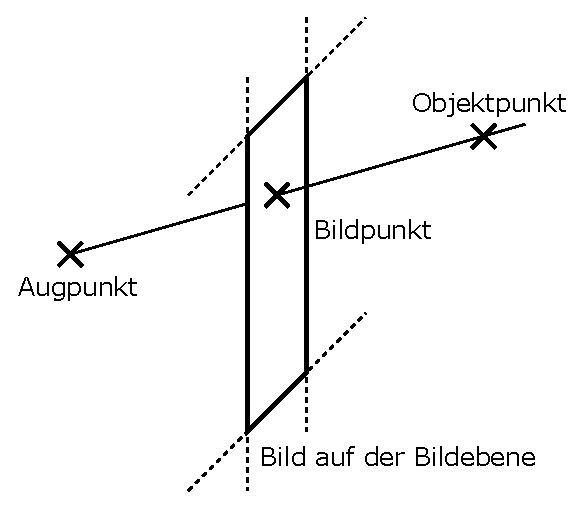
\includegraphics[width=\textwidth]{includes/perspective}
	\end{subfigure}
	\hfill
	\begin{subfigure}{0.4\textwidth}
		
\includegraphics[width=\textwidth]{includes/perspective2}
	\end{subfigure}
	\caption{Perspektivische Projektion}
	\label{fig:perspective}
\end{figure}

Oft wird die perspektivische Projektion in Verbindung mit Bildern, wie sie in \Fref{sec:imagecoordinates} beschrieben werden, verwendet, und nicht mit konkreten Bildpunkten. Dazu muss definiert werden, wo sich das Bild auf der Bildebene befindet. Eine offensichtliche Möglichkeit ist die Angabe der Höhe und Breite des Bildes auf der Bildebene, unter der Annahme, dass der am nächsten liegende Punkt der Bildebene zum Augpunkt in der Mitte des Bildes liegt. Wenn das Seitenverhältnis des Bildes beibehalten wird, reicht auch die Angabe der Höhe. Meistens ist es nicht relevant, wo sich die Bildebene genau befindet, sofern jedem Punkt eine Projektionsgerade zugeordnet wird, daher kann die Brennweite nach belieben verändert werden, solange auch die Bildhöhe entsprechend angepasst wird. Aus diesem Grund reicht es oft, nur die Brennweite als Parameter für die Projektion zu nutzen, sofern die Bildhöhe zuvor fest definiert wurde.

Angenommen das Bild ist $2$ Einheiten hoch, der Augpunkt ist $O(0,0,0)$ und die Kamera schaut in Richtung der negativen $z$-Achse. Dann kann aus den normalisierten Bildkoordinaten $(u,v)$ der entsprechende Bildpunkt $X'$ ganz einfach über die folgende Gleichung bestimmt werden:
\[ \vec{x'} = \begin{pmatrix}
u \\ v \\ -f
\end{pmatrix} \]

Alternativ zur Brennweite und Bildhöhe wird auch oft das vertikale \ac{FOV} benutzt, um die Projektion zu definieren. Das vertikale \ac{FOV} ist der Winkel zwischen den obersten und untersten Projektionsgeraden des Bildes. Die Brennweite $f$, die Bildhöhe $g$ und das vertikale \ac{FOV} $\fov$ stehen dabei in der folgende Beziehung:
\begin{align*}
	\fov = 2 \cdot \arctan \left( \frac{g}{2 f} \right)
	\Leftrightarrow f = \frac{g}{2 \tan\left(\frac{\fov}{2}\right)}
\end{align*}

\subsection{Triangulation}

Das Prinzip der Triangulation ist es aus zwei Eckpunkten und den Innenwickeln eines Dreiecks den dritten Eckpunkt zu bestimmen. Hier wird der Objektpunkt auf der Laserlinie auf Basis eines Bildpunktes und der Laserausrichtung bestimmt.

\subsubsection{Modell und gegebene Werte}

\begin{figure}
	\centering
	\begin{subfigure}{0.55\textwidth}
		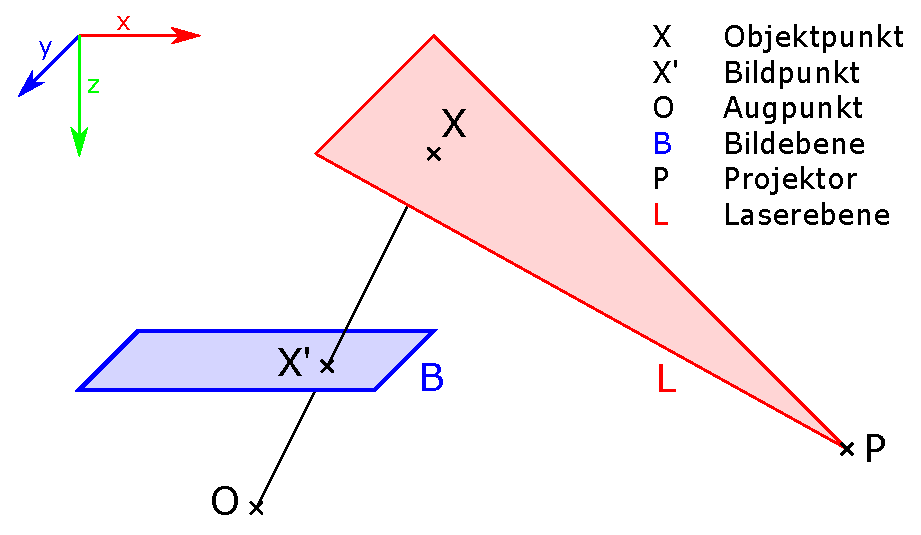
\includegraphics[width=\textwidth]{includes/triangulation3d}
		\caption{dreidimensionales Modell}
		\label{fig:triangulation3d}
	\end{subfigure}
	\hfill
	\begin{subfigure}{0.35\textwidth}
		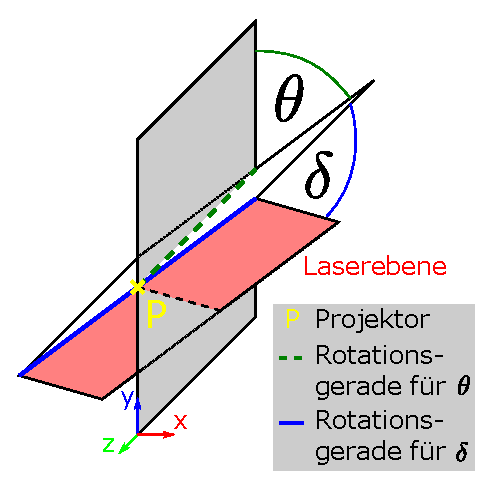
\includegraphics[width=\textwidth]{includes/triangulation_skew_pitch}
		\caption{Ausrichtung der Laserebene L}
		\label{fig:triangulation_skew_pitch}
	\end{subfigure}

	\begin{subfigure}{0.45\textwidth}
		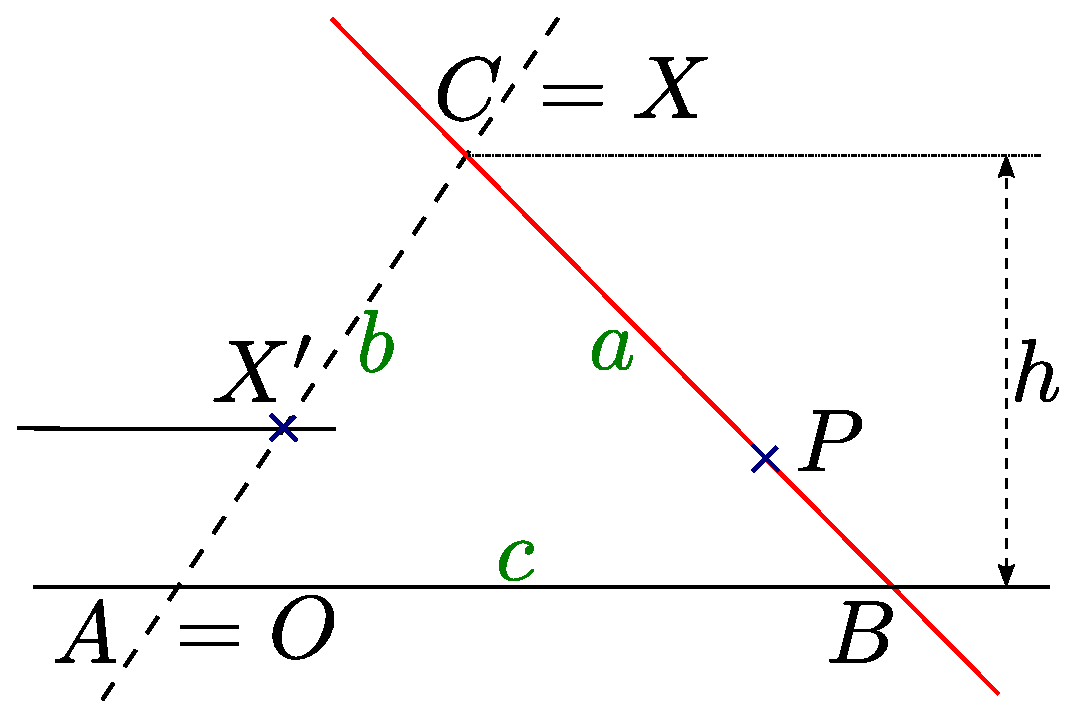
\includegraphics[width=\textwidth]{includes/triangulation2d}
		\caption{vereinfachtes zweidimensionales Modell}
		\label{fig:triangulation2d}
	\end{subfigure}
	\caption{Modell des Setups}
\end{figure}

Als Modell für die Triangulation wird die Abstraktion, wie sie auf \Fref{fig:triangulation3d} zu sehen ist, verwendet. Es existiert eine perspektivischen Projektion eines Objektpunktes $X$ auf eine Bildebene $B$, wobei die Blickrichtung entlang der negativen $z$-Achse verläuft. Der Augpunkt $O$ liegt dabei im Koordinatenursprung. Der Bildpunkt wird mit $X'$ bezeichnet. Das projizierte Licht wird durch eine Ebene $L$ dargestellt, die die Position des Projektors, das heißt den Projektionspunkt $P$, und den Objektpunkt $X$ schneidet.

Die durch das Setup gegebenen Werte:

\begin{tabular}{lp{12cm}}
	$P$                &
		Position des Linienprojektors.\\[0.5em]
	$f$                &
		Brennweite
		(unter der Annahme, dass das Bild auf der Bildebene $2$ Einheiten hoch ist)\\[0.5em]
	$\theta$,$\delta$  &
		Winkel zur Ausrichtung der Ebene $L$. Die Ausgangslage der Ebene ist parallel zur $y$-$z$-Ebene. Die Ebene wird zunächst mit dem Winkel $\theta$ um den Vektor {\color{red} $(0,0,-1)^T$} gedreht. Danach mit dem Winkel $\delta$ um den Vektor {\color{red} $(-\sin(\theta), -\cos(\theta), 0)^T$}. Siehe auch \Fref{fig:triangulation_skew_pitch}.
\end{tabular}

Zudem ist der Bildpunkt durch normalisierte Bildkoordinaten $(u, v)$ gegeben. Da die Brennweite $f$ auf eine Bildhöhe von $2$ Einheiten angepasst ist, gilt wie in \Fref{sec:perspective} beschrieben $X'(u, v, -f)$.

\subsubsection{Bestimmung der Entfernung}

Als \emph{Entfernung des Objektpunktes} $h$ wird die negierte 3. Koordinate von $X$ bezeichnet.

Um diese Entfernung zu bestimmen, wird das geometrische Modell des Setups vereinfacht. Als erstes wird ein Basiswechsel auf die Orthogonalbasis
\[ \left\lbrace \begin{pmatrix}
\cos(\theta) \\ \sin(\theta) \\ 0
\end{pmatrix}, \begin{pmatrix}
0 \\ 0 \\ -1
\end{pmatrix}, \begin{pmatrix}
\sin(\theta) \\ \cos(\theta) \\ 0
\end{pmatrix} \right\rbrace \]
vorgenommen, um im folgenden nur die ersten beiden Dimensionen zu betrachten. Der konstruierte zweidimensionale Raum hat die besondere Eigenschaft, dass von der Ebene $L$ und der $x$-$y$-Ebene nur die Geraden $a$ und $c$ übrig bleiben. Eine weitere besondere Eigenschaft ist, dass der Abstand zwischen $X$ und der $x$-$y$-Ebene direkt von einen in den anderen Raum übernommen werden kann. So entspricht $h$ im vereinfachten Modell der 2. Koordinate von $X$. Ein beliebiger Vektor $(v_1, v_2, v_3)^T$ im dreidimensionalen Model entspricht im zweidimensionalen Modell dem Vektor $(\cos(\theta) \cdot v_1 - \sin(\theta) \cdot v_2, -v_3)^T$.

Die Geraden $a$ und $c$ bilden zusammen mit der Geraden $b$, welche durch die Punkte $O$, $X$ und $X'$ verläuft, ein Dreieck, dessen Eckpunkte $A$, $C = X$ und $B = O$ sind. Dies ist auch nochmal in \Fref{fig:triangulation2d} zu sehen. Angenommen die Koordinaten von $P$ und $X'$ in der zweidimensionalen Darstellung sind $(p_1,p_2)$ und $(x'_1, x'_2)$, so können die Winkel $\alpha$ und $\beta$ und die Länge der Strecke zwischen $A$ und $B$ wie folgt berechnet werden:
\begin{align*}
	\alpha &= \frac{\pi}{2} - \arctan\left(\frac{x'_1}{x'_2}\right)\\
	\beta &= \frac{\pi}{2} + \delta\\
	\overline{AB} &= p_1 + \tan(\delta) \cdot p_2
\end{align*}

Die Entfernung $h$ ergibt sich daraufhin aus der folgenden Gleichung:
\[ h = \frac{\overline{AB} \cdot \sin(\alpha) \cdot \sin(\beta)}{\sin(\pi - \beta - \alpha)} \]

\subsubsection{Bestimmung der Koordinaten}

Nachdem die Entfernung $h$ des Objektpunktes bekannt ist, kann der Objektpunkt $X$ aus dem Bildpunkt bestimmt werden:
\[ \vec{x} = \frac{h}{f} \cdot \vec{x'} = \frac{h}{f} \cdot \begin{pmatrix}
u \\ v \\ -f
\end{pmatrix} \]

% ---------------------------------------------------------------------------- %

\section{Aufbau und Algorithmen}
\label{sec:realization}

\subsection{Hardware}

Die Hardware besteht aus einer Webcam und einem Low Cost Linienlaser, der auf einem Modellbauservo montiert ist. Laser und Servo werden von einem Mikrocontroller gesteuert, welcher wiederum über USB mit der Software kommuniziert. Der Aufbau ist in der Abbildung~\ref{fig:hardware} zu sehen. Alle diese Komponenten sind zusammen für unter 100\,€ erhältlich.

\begin{figure}
	\centering
	\begin{subfigure}{0.45\textwidth}
		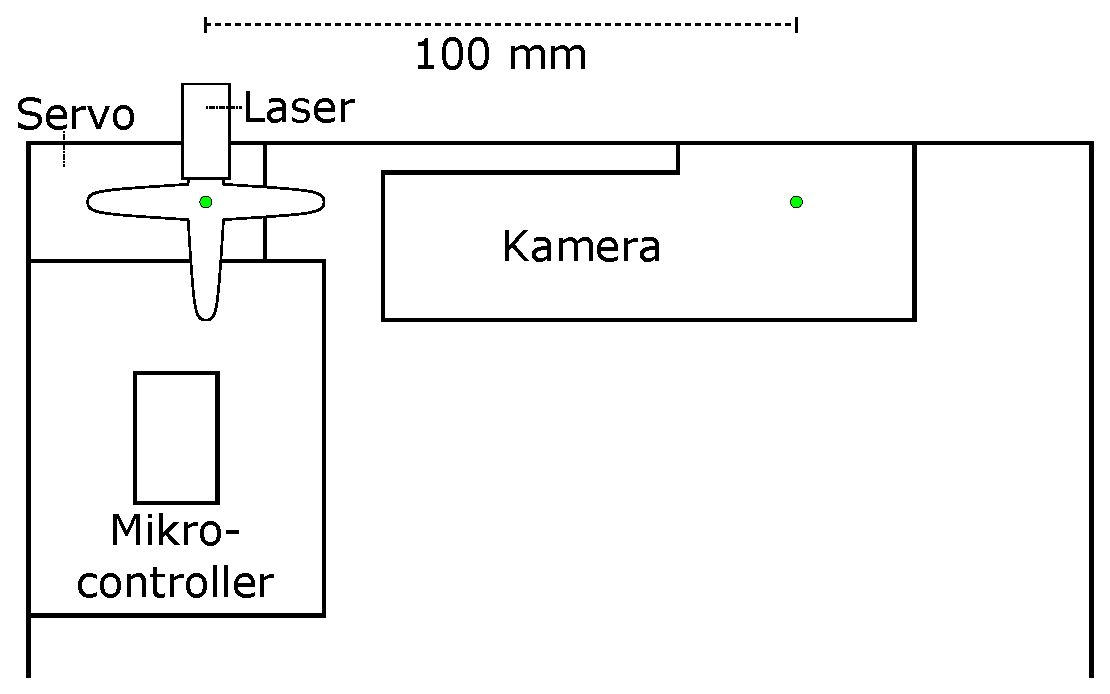
\includegraphics[width=\textwidth]{includes/hardware_schematic}
		\caption{schematische Darstellung}
	\end{subfigure}
	\hfill
	\begin{subfigure}{0.45\textwidth}
		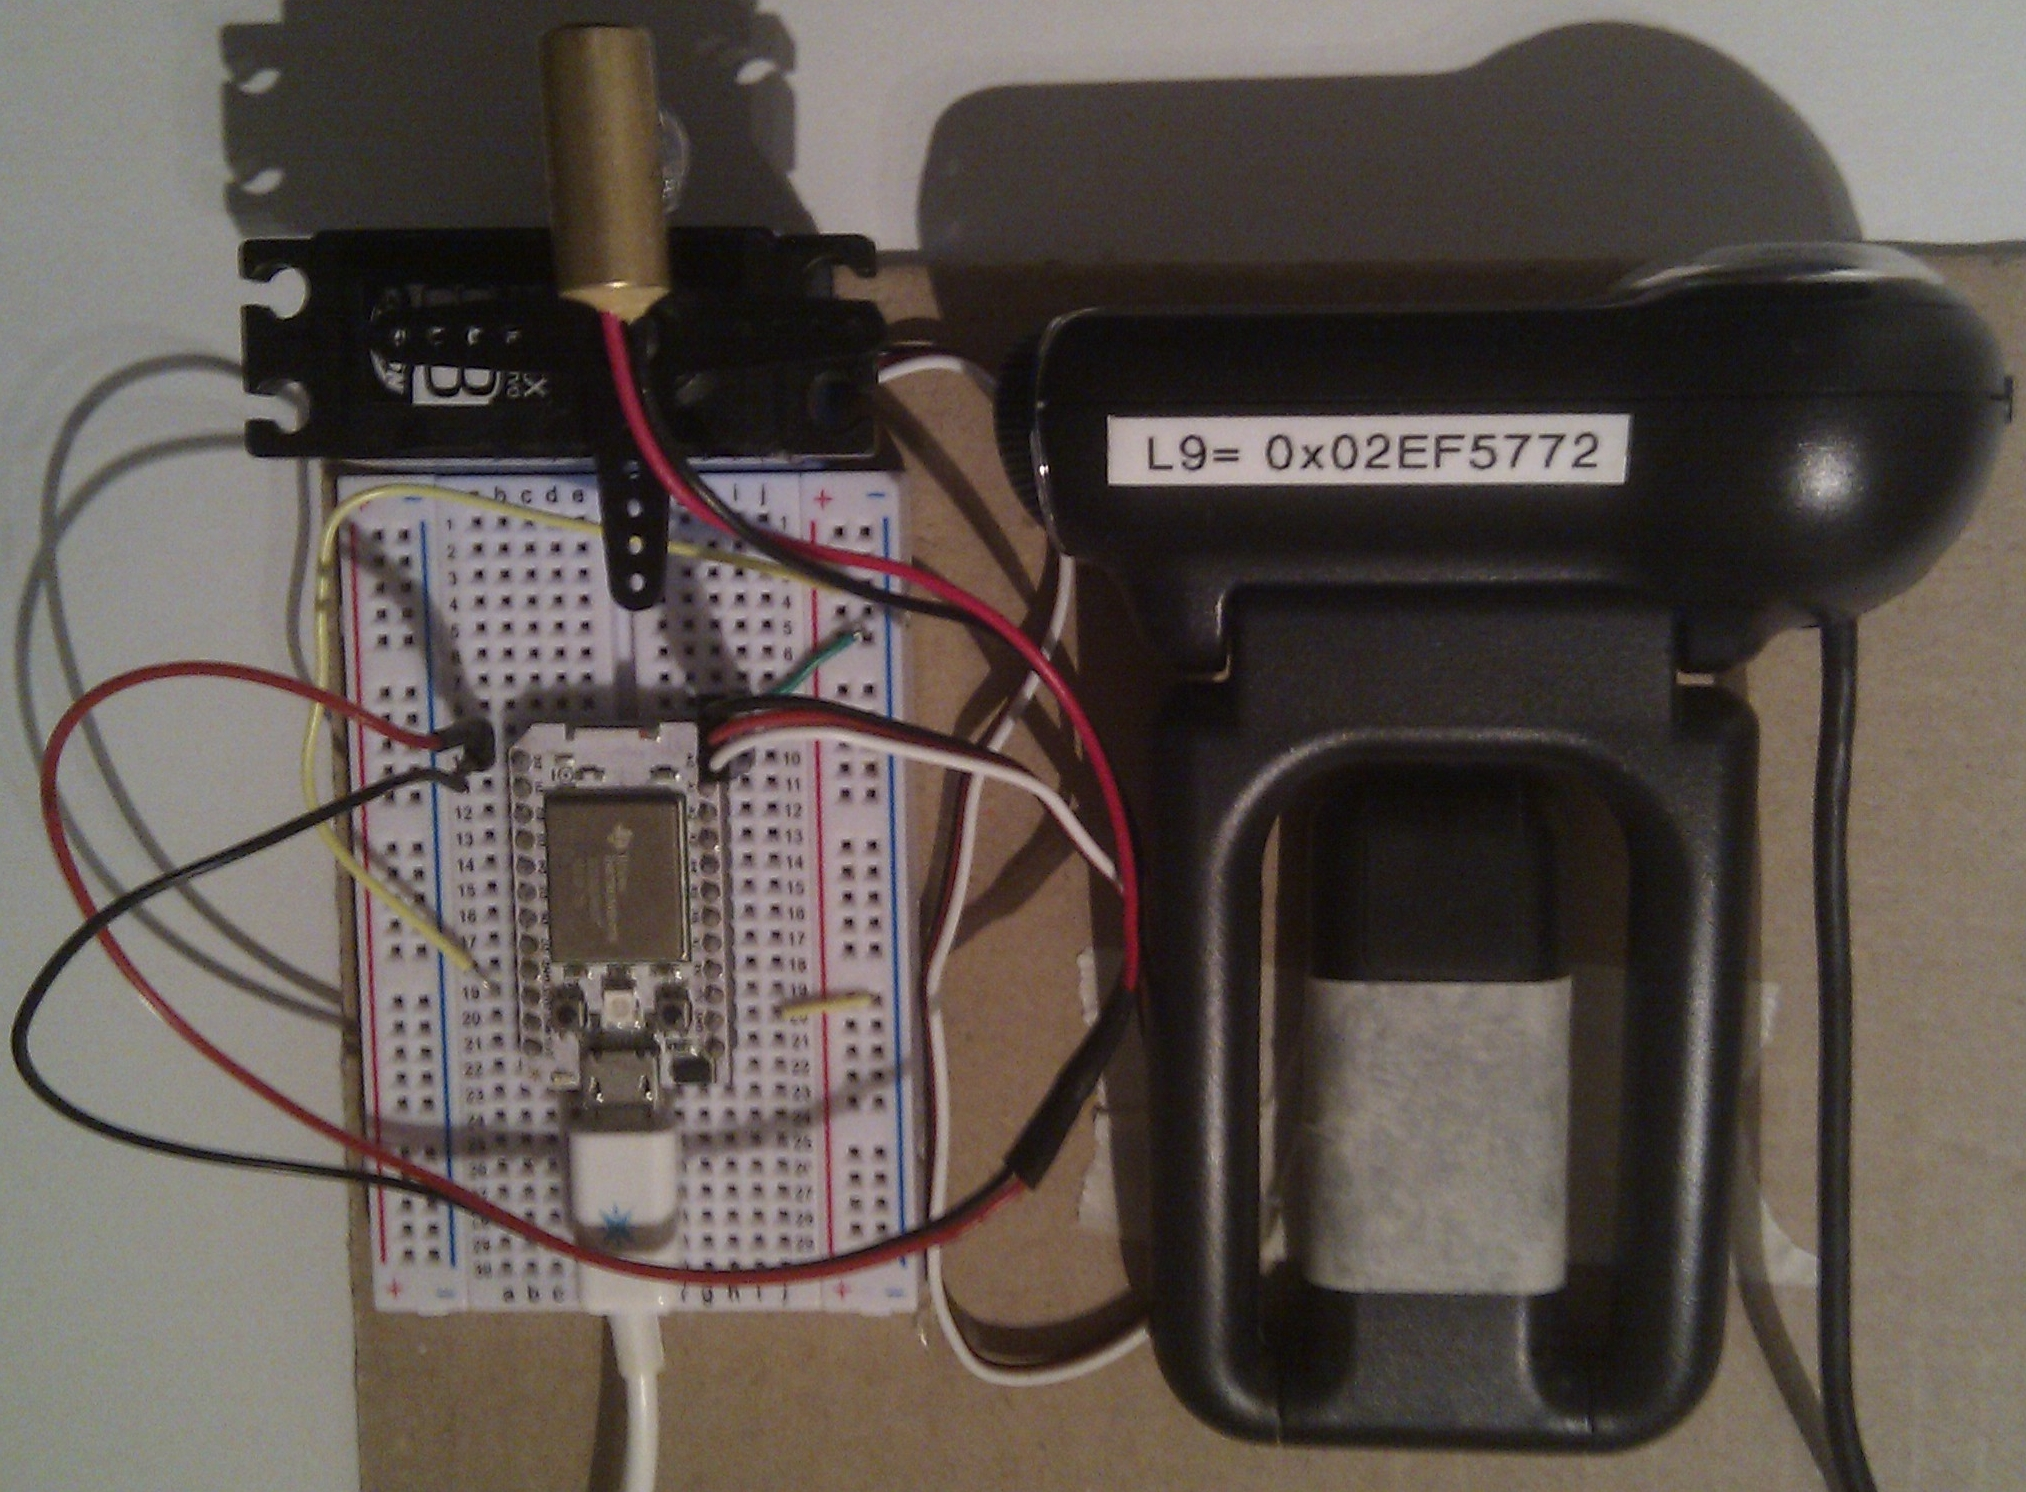
\includegraphics[width=\textwidth]{includes/hardware}
		\caption{reale Hardware}
	\end{subfigure}
	\caption{Aufbau der Hardware}
	\label{fig:hardware}
\end{figure}

\subsection{Softwarearchitektur}

Zur Implementierung der Software wurde die Programmiersprache \emph{C++} nach dem \emph{Standard von 2011} verwendet. Als Bibliotheken kamen \emph{OpenCV} und \emph{Qt} zum Einsatz. Eine Übersicht über alle Klassen ist in der Abbildung~\ref{fig:classes_all} zu finden. Im folgenden werden die einzelnen Komponenten der Software genauer betrachtet.

\begin{figure}[p]
	\centering
	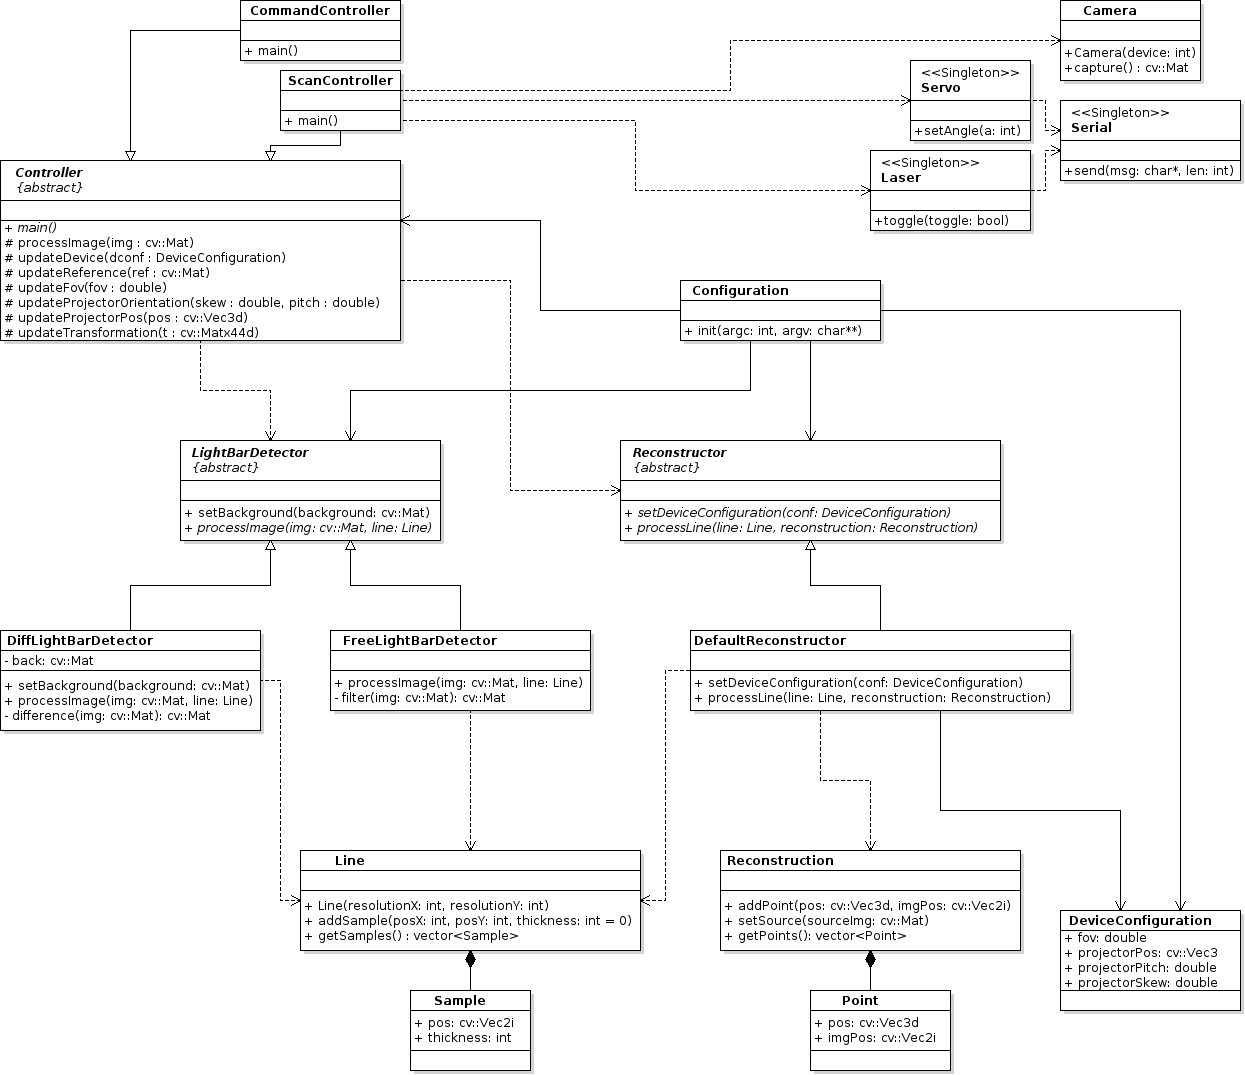
\includegraphics[width=\linewidth]{includes/classdiagram}
	\caption{Umfassendes Klassendiagramm}
	\label{fig:classes_all}
\end{figure}

\subsubsection{Grundlegende Datenstrukturen}

Zur Übertragung von Informationen zwischen den verschiedenen Komponenten werden die Datenstrukturen \texttt{Line}, \texttt{Reconstruction} und \texttt{DeviceConfiguration} verwendet. In \Fref{fig:classes_base} sind die entsprechenden Klassen zu sehen. Die Funktion wird im folgenden etwas genauer beschrieben.

\begin{figure}
	\centering
	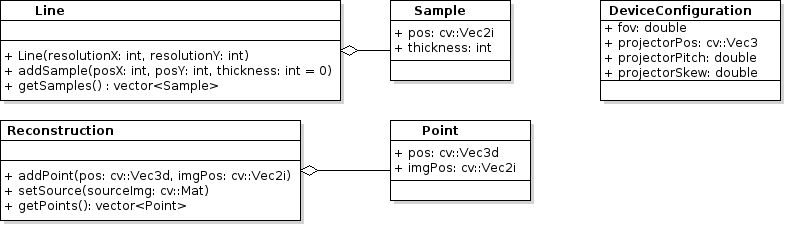
\includegraphics[width=\linewidth]{includes/classdiagram_base.png}
	\caption{Klassendiagramm zu den grundlegenden Datenstrukturen}
	\label{fig:classes_base}
\end{figure}

\vspace{0.5em}
\begin{tabular}{lp{10cm}}
	\texttt{DeviceConfiguration} &
		Die Struktur \texttt{DeviceConfiguration} speichert alle Werte zum Setup, die zur Rekonstruktion benötigt werden. Zusätzlich wird eine Transformationsmatrix mitgeführt, auf die später noch eingegangen wird.\\[1em]
	\texttt{Line}                &
		Die Datenstruktur \texttt{Line} entspricht einer Menge von Abtastungen der projizierten Linie. Sie Speichert dabei zusätzlich zu einer Liste von Abtastungen (Instanzen von \texttt{Sample}) die Auflösung des zugrunde liegenden Bildes.\\[1em]
	\texttt{Reconstruction}      &
		Die Klasse \texttt{Reconstruction} dient zum Speichern des endgültigen Ergebnisses der Rekonstruktion. Sie speichert somit eine Liste von rekonstruierten Punkten (Instanzen von \texttt{Point}). Zusätzlich hat die Klasse die Aufgabe, hinzugefügte rekonstruierte Punkte zur Ausgabe des Programms hinzuzufügen. Die entsprechenden Farben werden aus dem Referenzbild entnommen.
\end{tabular}

\subsubsection{Programmablauf}

\begin{figure}
	\centering
	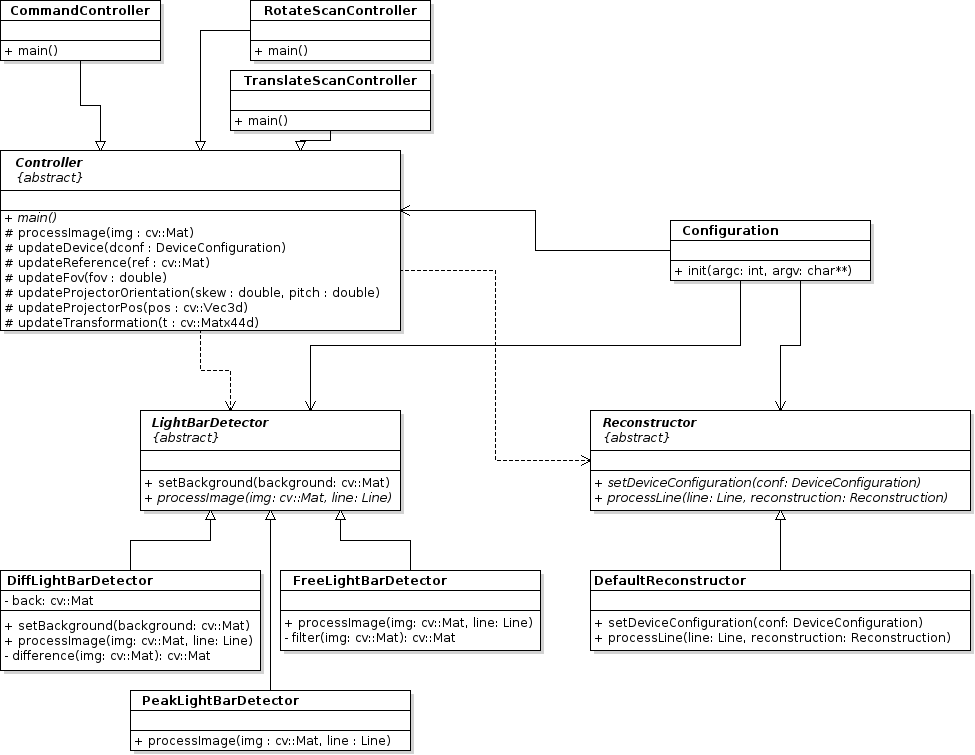
\includegraphics[width=\linewidth]{includes/classdiagram_control.png}
	\caption{Klassendiagramm zu den Steuereinheiten}
	\label{fig:classes_control}
\end{figure}

Nach Programmstart wird als erstes die Funktion \texttt{Configuration::init(int,char**)} aufgerufen. Diese analysiert die Argumente, die dem Programm übergeben wurden, und speichert das Ergebnis in den statischen Feldern der Klasse. Unter anderem wird dabei jeweils eine Instanz einer Spezialisierung von \texttt{Controller}, \texttt{LightBarDetector} und \texttt{Reconstructor} in den Feldern von \texttt{Configuration} abgelegt. Als nächstes wird die Methode \texttt{main()} der \emph{Steuerungsklasse}, also der Spezialisierung von \texttt{Controller}, aufgerufen, welche den Rest des Programmablaufes steuert.

\subsection{Steuerungsklassen}
\label{sec:controller}

\begin{figure}
	\centering
	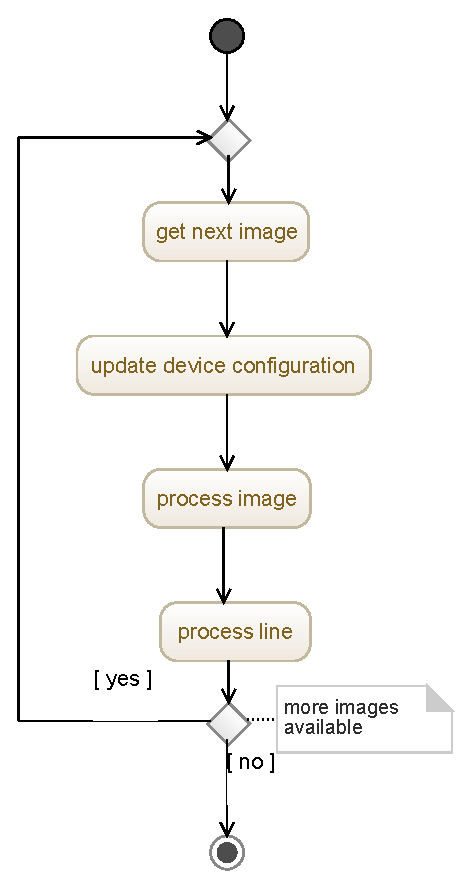
\includegraphics[width=0.4\linewidth]{includes/software_controller}
	\caption{Aktivitätsdiagramm zum Grundlegenden Programmablauf in den Steuerklassen.}
	\label{fig:software_controller}
\end{figure}

Der Ablauf, der von den verschiedenen Spezialisierungen von \texttt{Controller} vorgegeben wird, verfolgt dabei immer einen ähnlichen Ablauf, wie er auch in Abbildung~\ref{fig:software_controller} dargestellt wird. Der Controller durchläuft eine Schleife und beschafft sich in jedem Schleifendurchlauf die aktuelle Gerätekonfiguration (\texttt{DeviceConfiguration}), eine Aufnahme durch das entsprechende Setup und ggf. ein aktuelles Referenzbild. Danach übergibt es die Steuerung an die Linienerkennung (\texttt{LightBarDetextor}) und dessen Ergebnis wird an den Rekonstruktionsalgorithmus (\texttt{Reconstructor}) übergeben.

Es existieren drei Spezialisierungen von \texttt{Controller}. Die einfachste Implementierung ist der \texttt{CommandController}, welcher Standardmäßig verwendet wird. Die Klasse liest die Standardeingabe oder die in den Argumenten definierte Datei Zeilenweise aus. Eine Zeile entspricht dabei einem Befehl, welcher ausgewertet und ausgeführt wird, bevor sich das Programm der nächsten Zeile zuwendet. In der Tabelle~\ref{tab:commands} können alle Befehle nachgelesen werden.

\begin{table}[p]
	\centering
	\begin{tabular}{lp{10cm}}
		\bfseries Befehl             & \bfseries Beschreibung\\
		\hline\hline
		\texttt{b <Datei>}           &
			Diese Zeile definiert die angegebene \emph{Datei} als neues Referenzbild.\\
		\hline
		\texttt{fov <Winkel>}        &
			Hier wird das \ac{FOV} auf den angegebenen \emph{Winkel} gesetzt. Der Winkel muss dabei in Radiant angegeben werden.\\
		\hline
		\texttt{pp <x> <y> <z>}      &
			Der Befehl setzt die Projektorposition $P$ auf den Punkt $(x,y,z)$.\\
		\hline
		\texttt{po <skew> <pitch>}   &
			Setzt die Werte $\theta$ und $\delta$ aus dem Modell. Die Winkel müssen dabei in Radiant angegeben werden.\\
		\hline
		\texttt{t <$m_1$> \dots <$m_{16}$>} &
			Setzt die Transformationsmatrix. Dabei wird die Matrix Zeilenweise aufgefüllt:
			\[ \begin{pmatrix}
				m_{1}  & m_{2}  & m_{3}  & m_{4}\\
				m_{5}  & m_{6}  & m_{7}  & m_{8}\\
				m_{9}  & m_{10} & m_{11} & m_{12}\\
				m_{13} & m_{14} & m_{15} & m_{16}
			\end{pmatrix} \]\\
		\hline
		\texttt{c <x> <fov> <pitch>} &
			Setzt die Projektorposition $P$ auf $(x,0,0)$, das \ac{FOV} auf den angegeben Winkel $\fov$, $\delta$ auf den angegeben Wert von \emph{pitch} und $\theta = 0$.\\
		\hline
		\texttt{<Datei>}             &
			Lässt die Rekonstruktion auf Basis der angegebenen Aufnahme laufen.\\
		\hline\hline
	\end{tabular}
	\caption{Unterstützte Befehle der Steuerungsklasse \texttt{CommandController}.}
	\label{tab:commands}
\end{table}

Die Klassen \texttt{RotateScanController} und \texttt{TranslateScanController} beschaffen die Aufnahmen hingehen direkt von der Hardware. Der \texttt{RotateScanController} rotiert dabei den Streifenprojektor um passende Aufnahmen zu erhalten. Der \texttt{TranslateScanController} macht eine Aufnahme und wartet anschließend auf eine Bestätigung des Benutzers, dass sich das zu scannende Objekt um eine vorher definierte Strecke bewegt hat, bevor er das nächste Bild aufnimmt.

\subsection{Ansteuerung der Hardware}

\subsubsection{Ansteuerung des Mikrocontrollers}

Die Software steuert den Mikrocontroller über USB, wobei sich dieser als virtuellen COM-Port ausgibt. Zur Kommunikation wird ein einfaches Protokoll verwendet, das 2 Byte lange Nachrichten an den Mikrocontroller sendet. Das erste Byte gibt den Befehl an, das zweite den Parameter. Die möglichen Befehle werden in der Tabelle~\ref{tab:protocol} aufgeführt.

\begin{table}
	\centering
	\begin{tabular}{|c|c|c|}
		\hline
		1. Byte & 2. Byte & Beschreibung \\
		\hline
		'm' & $\alpha \in [0,180]$ & Setzt die Servoposition auf $\alpha^\circ$\\
		\hline
		'l' & '0' oder '1' & Schaltet den Laser an ('1') bzw. aus ('0')\\
		\hline
	\end{tabular}
	\caption{Befehle zur Steuerung des Mikrocontrollers. Zeichen in einfachen Anführungszeichen stehen für den ASCII-Wert des Zeichens.}
	\label{tab:protocol}
\end{table}

Die Klasse \texttt{Serial} ermöglicht es Nachrichten an den Mikrocontroller zu senden. Die Klassen \texttt{Servo} und \texttt{Laser} implementieren die Steuerung von dem Servo bzw. Laser. Dabei werden Nachrichten in o.g. Form an den Mikrocontroller gesendet.

\subsubsection{Ansteuerung der Kamera}

Für das Auslesen von Bildern der Kamera ist die Klasse \texttt{Camera} zuständig, dabei liest ein extra Thread permanent Bilder von der Kamera.

Wenn ein anderer Thread die \texttt{capture}-Methode von \texttt{Camera} aufruft, blockiert er solange, bis der extra Thread das nächste Bild gelesen hat, und gibt dieses dann zurück. Das wird gemacht um sicherzustellen, dass immer das aktuellste Bild ausgelesen wird und nicht ein älteres Bild, das in einem Buffer der Kamera gespeichert wurde.


\subsection{Linienerkennung}

Die Linienerkennung arbeitet in zwei Schritten. Zuerst wird ein Binärbild erzeugt, wobei der Algorithmus entscheidet, welche Pixel zur Linie gehören und welche nicht. Im zweiten Schritt wird jeder Pixel des Bild durchlaufen, wobei in der Datenstruktur \texttt{Line} die vermeintliche Position der Linie und deren Breite gespeichert wird. Die hier implementierten Algorithmen unterscheiden sich lediglich in der Erzeugung des Binärbildes.

\subsubsection{Differenzbildung (Diff)}

Bei diesem Verfahren muss für jedes zu analysierende Bild ein Referenzbild ohne die projizierte Linie gegeben sein. Dabei wird die Differenz für jedes Bild mit dem Referenzbild berechnet und mit Hilfe eines einfachen Filters in ein Binärbild umgewandelt.

\subsubsection{Farbfilter (Free)}

Für jeden Farbkanal wird einzeln der Mittelwert über das gesamte Bild berechnet, aus dem ein Schwellenwert für jeden Kanal einzeln bestimmt wird. Für jeden Pixel wird der Wert aller Farbkanäle mit dem Schwellenwert verglichen. Ist ein Wert kleiner als der entsprechende Schwellenwert, gehört der Pixel nicht zur Linie.

\subsection{Rekonstruktion}

Nachdem die Laserlinie erkannt wurde, werden die vermeintlichen Pixel der erkannten Linie in Objektpunkte überführt. Dies geschieht durch die Klasse \texttt{DefaultReconstructor}, welche derzeit die einzige Spezialisierung von \texttt{Reconstructor} darstellt.

Dazu werden die Formeln aus \Fref{sec:basics} angewendet, um für jeden Pixel zunächst die normalisierten Bildkoordinaten, die Entfernung $h$ und danach den Objektpunkt $X$ zu bestimmen. Daraufhin werden die erhalten Punkte mithilfe der Transformationsmatrix transformiert und an die Klasse \texttt{Reconstruction} weiter gegeben, welche sie letztendlich ausgibt.
	
%\begin{table}[p]
%	\centering
%	\begin{tabular}{lp{10cm}}
%		\bfseries Klasse                & \bfseries Funktion\\
%		\hline\hline
%		\texttt{CommandController}      &
%			Diese Klasse stellt als Spezialisierung von \texttt{Controller} eine Steuerungsklasse da, welche eingehende Befehle verarbeitet. Eine Liste der Befehl ist in \Fref{tab:commands} zu finden.\\
%		\hline
%		\texttt{Configuration}          &
%			Diese Klasse ist eine rein statische Klasse. Sie analysiert nach Programmstart die Argumente, die an das Programm übergeben wurden, und speichert die Einstellungen für die weitere Programmausführung.\\
%		\hline
%		\texttt{Controller}             &
%			Diese abstrakte Klasse bildet die Basis für alle Steuerungsklassen und definiert Funktionen mit denen die Steuerungsklasse ihre Arbeit verrichten kann. Eine Steuerungsklasse bestimmt den Programmablauf und ist dabei für die Beschaffung der Setup-Informationen und Bilder verantwortlich.\\
%		\hline
%		\texttt{DefaultReconstructor}   &
%			Als Spezialisierung von \texttt{Reconstructor} stellt diese Klasse den einzigen Rekonstruktionsalgorithmus da.\\
%		\hline
%		\texttt{DeviceConfiguration}    &
%			Diese Struktur speichert alle Werte zum Setup, die zur Rekonstruktion benötigt werden. Dazu gehört beispielsweise die Position und Ausrichtung des Projektors. Zusätzlich wird eine Transformationsmatrix mitgeführt, auf dessen Basis Punkte nach der Triangulation transformiert werden.\\
%		\hline
%		\texttt{DiffLightBarDetector}   &
%			Als Spezialisierung von \texttt{LightBarDetector} stellt diese Klasse eine Linienerkennung da.  Nähere Informationen in \Fref{sec:line_diff}.\\
%		\hline
%		\texttt{FreeLightBarDetector}   &
%			Als Spezialisierung von \texttt{LightBarDetector} stellt diese Klasse eine Linienerkennung da. Nähere Informationen in \Fref{sec:line_free}.\\
%		\hline
%		\texttt{LightBarDetector}       &
%			Diese abstrakte Klasse dient als Basis für alle Implementierungen zur Detektion der Laserlinie.\\
%		\hline
%		\texttt{Line}                   &
%			Diese Datenstruktur entspricht einer Menge von Abtastungen der projizierten Linie. Sie Speichert dabei eine Liste von Indices, dessen Pixel zur Laserlinie gehören, und die Auflösung des zugrunde liegenden Bildes. Die Indices werden dabei in Instanzen von \texttt{Sample} abgelegt.\\
%		\hline
%		\texttt{Reconstruction}         &
%			Diese Klasse speichert das endgültige Ergebnis der Rekonstruktion. Außerdem kümmert sie sich um die Ausgabe der rekonstruierten Punkte.\\
%		\hline
%		\texttt{Reconstructor}          &
%			Diese abstrakte Klasse dient als Basis für alle Implementierungen zur Rekonstruktion der Objektpunkte auf Basis der bereits erkannten Laserlinie.\\
%		\hline
%		\texttt{RotateScanController}   &
%			Diese Klasse stellt als Spezialisierung von \texttt{Controller} eine Steuerungsklasse da. Sie kann verwendet werden, um Objekte mit Hilfe einer Drehung des Projektors zu scannen.\\
%		\hline
%		\texttt{TranslateScanController} &
%			Diese Klasse stellt als Spezialisierung von \texttt{Controller} eine Steuerungsklasse da. Sie kann verwendet werden, um Objekte mit Hilfe einer schrittweisen Bewegung an der Kamera vorbei zu scannen.\\
%		\hline\hline
%	\end{tabular}
%	\caption{Umfassende Tabelle der Klassen}
%	\label{tab:classes_all}
%\end{table}

% ---------------------------------------------------------------------------- %

\section{Auswertung}
\label{sec:evaluation}

Im Folgenden werden verschiedene Seiten eines ''Rubik's Cube'' auf verschiedene Entfernungen gescannt. Es wurden die rote, grüne, blaue, gelbe und orange Seite in 300mm Entfernung, sowie die blaue Seite in 200mm, 400mm und 500mm Entfernung vermessen. Die Zugehörigkeit eines Messpunktes wird anhand seiner Farbe, die aus dem Referenzbild entnommen wurde, bestimmt. Da die Scans vor weißem Hintergrund durchgeführt wurden, wurde die weiße Seite des ''Rubik's Cube'' nicht gescannt.



\begin{figure}[H]
	\centering
	\begin{subfigure}{0.45\textwidth}
		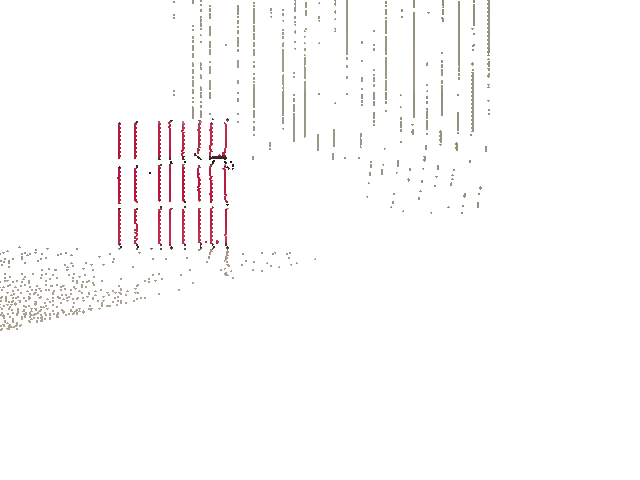
\includegraphics[width=\textwidth]{includes/diff_red_cam.png}
		\caption{komplette Punktwolke aus Sicht der Kamera}
	\end{subfigure}
	\hfill
	\begin{subfigure}{0.45\textwidth}
		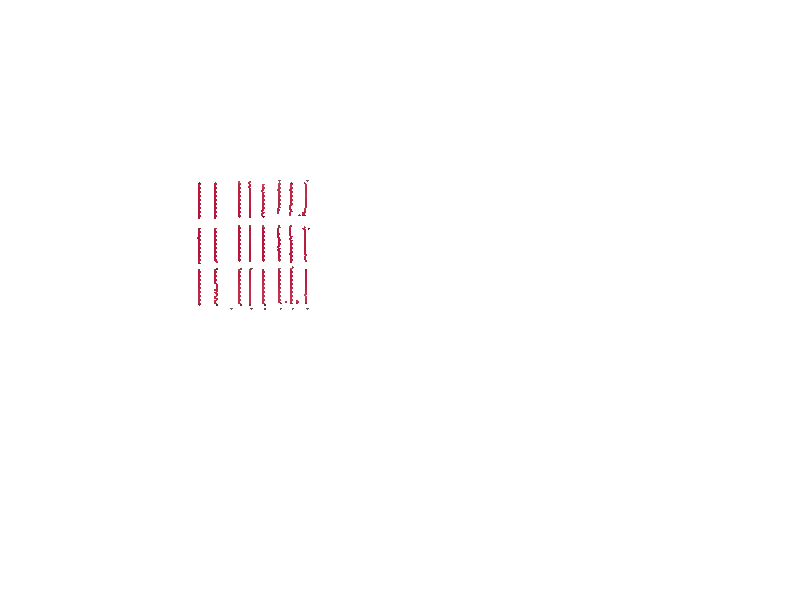
\includegraphics[width=\textwidth]{includes/diff_only_red_cam.png}
		\caption{Punktwolke der Punkte, die zum Würfel gehören, aus Sicht der Kamera}
	\end{subfigure}
	\begin{subfigure}{0.45\textwidth}
		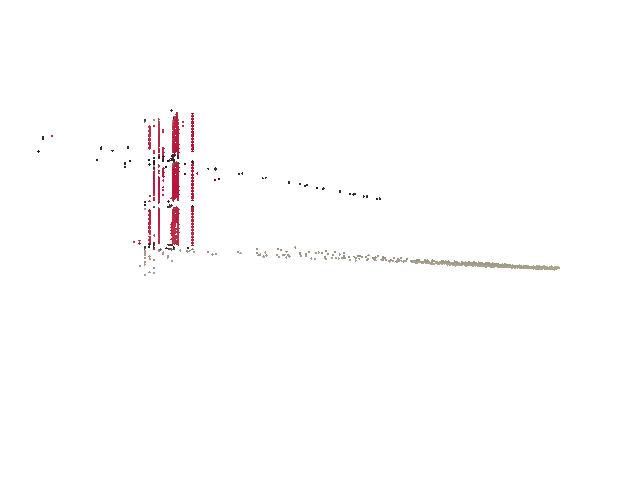
\includegraphics[width=\textwidth]{includes/diff_red_pos1.png}
		\caption{komplette Punktwolke von der Seite}
	\end{subfigure}
	\hfill
	\begin{subfigure}{0.45\textwidth}
		
\includegraphics[width=\textwidth]{includes/diff_only_red_pos1.png}
		\caption{Punktwolke der Punkte, die zum Würfel gehören, von der Seite}
	\end{subfigure}
	\caption{Punktwolken eines Scans mit diff-Linienerkennung der Orangen Seite des ''Rubic's Cube'' in 300mm Entfernung}
\end{figure}

\begin{figure}[H]
	\centering
	\begin{subfigure}{0.45\textwidth}
		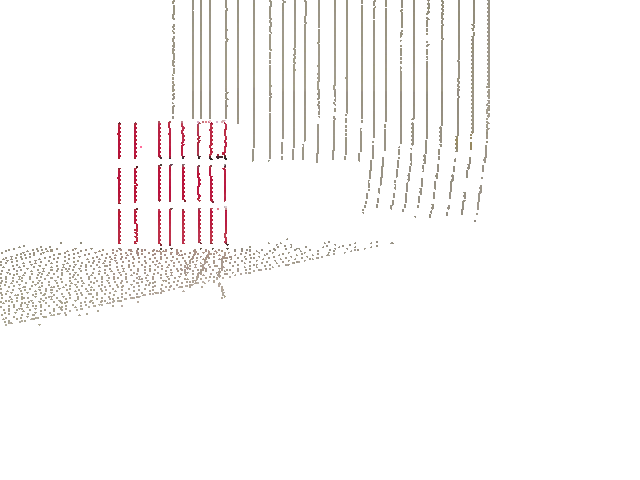
\includegraphics[width=\textwidth]{includes/free_red_cam.png}
		\caption{komplette Punktwolke aus Sicht der Kamera}
	\end{subfigure}
	\hfill
	\begin{subfigure}{0.45\textwidth}
		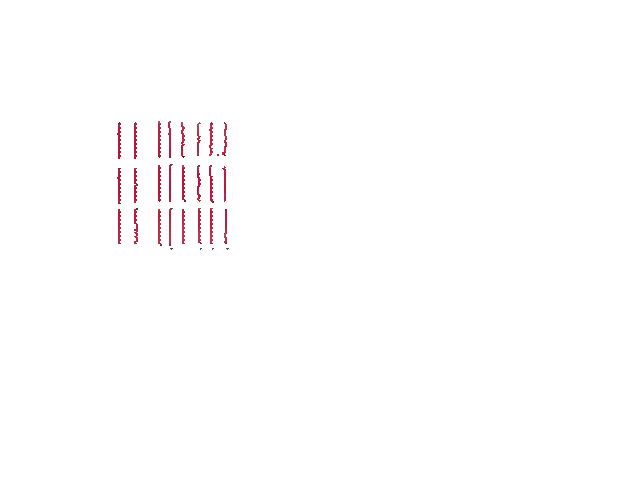
\includegraphics[width=\textwidth]{includes/free_only_red_cam.png}
		\caption{Punktwolke der Punkte, die zum Würfel gehören, aus Sicht der Kamera}
	\end{subfigure}
	\begin{subfigure}{0.45\textwidth}
		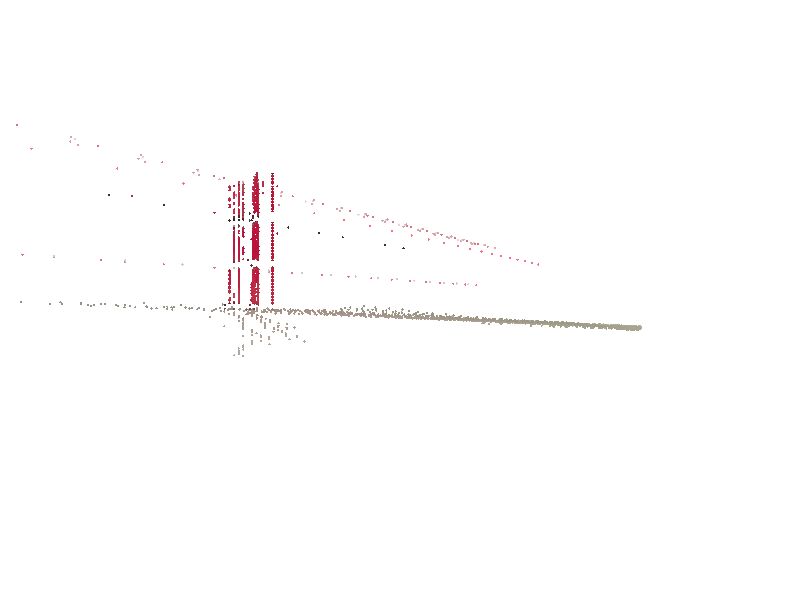
\includegraphics[width=\textwidth]{includes/free_red_pos1.png}
		\caption{komplette Punktwolke von der Seite}
	\end{subfigure}
	\hfill
	\begin{subfigure}{0.45\textwidth}
		
\includegraphics[width=\textwidth]{includes/free_only_red_pos1.png}
		\caption{Punktwolke der Punkte, die zum Würfel gehören, von der Seite}
	\end{subfigure}
	\caption{Punktwolken eines Scans mit free-Linienerkennung der Orangen Seite des ''Rubic's Cube'' in 300mm Entfernung}
\end{figure}


\subsection{Wiederholte Messungen}
\label{sec:reps}

Zunächst wurde die blaue Seite des ''Rubic's Cube'' zehn mal in 300mm Entfernung vermessen, um die Abweichungen zwischen zwei Messungen zu bestimmen. In Tabelle \ref{tab:reps} sind die Ergebnisse aufgeführt, wobei im linken Teil der Tabelle (''diff'') die Resultate nach diff-Linienerkennung und im rechten Teil (''free'') die nach free-Linienerkennung stehen. In der Spalte ''Anzahl'' steht jeweils die Anzahl der Punkte, die zum Würfel gehören, unter ''Avg'' ist das $20 \%$ gestutzte Mittel aller gemessenen Entfernungen und unter ''Stdabw'' die Standardabweichung der gemessenen Entfernungen.

Es fällt auf, dass sich die Werte zwischen verschiedenen Messungen kaum unterscheiden, aber es zwischen den beiden Linienerkennungen z.T. große Unterschiede gibt. So findet diff mehr als doppelt so viele Punkte auf dem Würfel und die Standardabweichung ist ca. fünf mal größer.

Wie man in Abbildung \ref{fig:blue_0_cam} sehen kann, spiegelt sich der Laser in dem Cube. Die diff-Linienerkennung (Abbildung \ref{fig:blue_0_diff}) erkennt, im Gegensatz zur free-Linienerkennung (Abbildung \ref{fig:blue_0_free}), die Spiegelung als Linie. Das erklärt sowohl warum diff mehr Punkte erkennt, als auch warum diese eine höhere Streuung aufweisen. Da die falsch erkannten Punkte überwiegend links von der tatsächlichen Linie liegen, haben sie eine kleinere Entfernung, was den etwas geringeren Durchschnitt von diff gegenüber free erklärt.

Zusätzlich fällt auf, dass die durchschnittliche Entfernung von sowohl diff als auch free 38mm - 41mm ($12,5\%-13,5\%$) größer ist als erwartet (300mm), siehe dazu Abschnitt \ref{sec:dists}.

\begin{table}[H]
	\centering
	\begin{tabular}{c|c|c}
		& diff & free \\
		\begin{tabular}{c}
			Wiederholung \\ \hline
			1 \\
			2 \\
			3 \\
			4 \\
			5 \\
			6 \\
			7 \\
			8 \\
			9 \\
			10 \\
		\end{tabular} & 
		\begin{tabular}{c|c|c}
			Anzahl & Avg (mm) & Stdabw (mm) \\ \hline
			825 & 338.851 & 15.1979 \\
			829 & 338.511 & 14.199 \\
			807 & 338.858 & 13.7228 \\
			818 & 338.825 & 15.9249 \\
			851 & 338.931 & 15.6883 \\
			857 & 338.927 & 13.3769 \\
			832 & 338.541 & 14.5219 \\
			847 & 338.688 & 14.5952 \\
			825 & 338.494 & 13.6795 \\
			830 & 338.469 & 16.8786 \\
		\end{tabular} &
		\begin{tabular}{c|c|c}
			Anzahl & Avg (mm) & Stdabw (mm) \\ \hline
			363 & 340.952 & 2.76884 \\
			365 & 340.923 & 2.97673 \\
			344 & 341.142 & 2.75016 \\
			336 & 341.02 & 2.68906 \\
			365 & 340.75 & 2.59545 \\
			350 & 340.738 & 2.71992 \\
			354 & 340.867 & 2.93117 \\
			353 & 340.764 & 2.9996 \\
			351 & 340.737 & 2.80947 \\
			354 & 341.064 & 2.97436 \\
		\end{tabular}
	\end{tabular}
	\caption{Scans der blauen Seite in 300mm Entfernung}
	\label{tab:reps}
\end{table}

\subsection{Verschiedene Farben}
\label{sec:cols}

Als nächstes wurden die verschiedenen Seiten des ''Rubic'c Cube'' gescannt, um die Farbabhängigkeit der Linienerkennungen zu überprüfen. Die Ergebnisse sind in Tabelle \ref{tab:colors} zu finden. Sie ist analog zur Tabelle \ref{tab:reps} aus Abschnitt \ref{sec:reps} aufgebaut, mit dem Unterschied, dass in pro Zeile nicht die Punkte aus einer Messung, sondern aus zehn Messungen betrachtet werden.

Es fällt auf, dass bei der roten Seite beide Linienerkennungen gute Ergebnisse liefern (niedrige Streuung der Messpunkte) und auch die Anzahl der gefunden Punkte und die Durchschnittsentfernung nahe beieinanderliegen. Zusätzlich liefern beide Linienerkennungen bei Gelb vergleichsweise schlechte Ergebnisse (hohe Streuung). Bei den anderen Farben unterscheiden sich die Linienerkennungen z.T. stark, so liefert diff bei grün die schlechtesten Ergebnisse, wohingegen free mit orange starke Probleme hat. Nicht nur die Standardabweichung ist bei orange und free extrem hoch, auch die Anzahl der gefundenen Punkte ist ungefähr acht mal größer als bei grün oder blau, das heißt, dass ca. $\frac{7}{8}$ der erkannten Punkte nicht zur Linie gehören, weil free den Mittelwert über das gesamte Bild bildet und anhand der Abweichung eines Punktes zum Mittelwert bestimmt, ob ein Punkt zur Linie gehört oder nicht. Die orange Seite sorgt verändert den Mittelwert so, dass auch Punkte, die nicht zur Linie gehören erkannt werden.

Insgesamt scheint diff farbunabhängiger zu sein, da die Durchschnittsentfernung ziemlich konstant ist und auch die Anzahl der gefundenen Punkte weniger stark schwankt, als bei free. 


\begin{table}[H]
	\centering
	\begin{tabular}{c|c|c}
		& diff & free \\
		\begin{tabular}{c}
			Farbe \\ \hline
			Rot \\
			Gruen \\
			Blau \\
			Gelb \\
			Orange \\
		\end{tabular} & 
		\begin{tabular}{c|c|c}
			Anzahl & Avg (mm) & Stdabw (mm) \\ \hline
			6565 & 338.14 & 3.6842 \\
			8806 & 337.897 & 88.2139 \\
			8321 & 338.722 & 14.8228 \\
			7085 & 338.112 & 39.4331 \\
			6336 & 338.249 & 7.50314 \\
		\end{tabular} & 
		\begin{tabular}{c|c|c}
			Anzahl & Avg (mm) & Stdabw (mm) \\ \hline
			6439 & 338.035 & 3.4453 \\
			3534 & 340.808 & 6.28125 \\
			3535 & 340.892 & 2.82819 \\
			10824 & 338.69 & 77.4283 \\
			29063 & 347.896 & 205.929 \\
		\end{tabular}
	\end{tabular}
	\caption{Scans der verschiedener Seiten in 300mm Entfernung}
	\label{tab:colors}
\end{table}


\begin{figure}[H]
	\centering
	\begin{subfigure}{0.32\textwidth}
		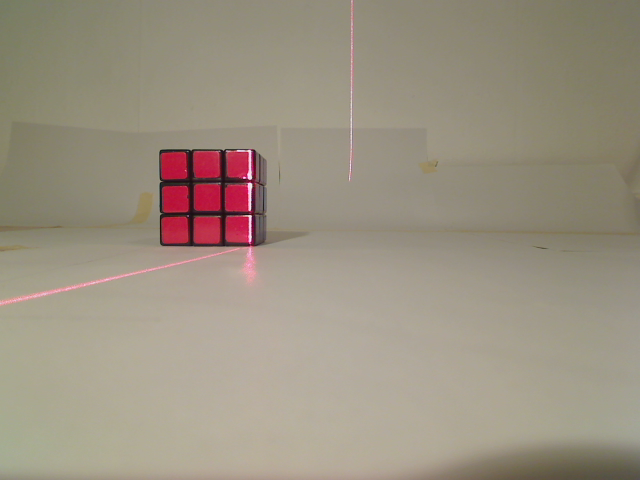
\includegraphics[width=\textwidth]{includes/red_0.png}
		\caption{Bild der Kamera\\}
		\label{fig:red_0_cam}
	\end{subfigure}
	\hfill
	\begin{subfigure}{0.32\textwidth}
		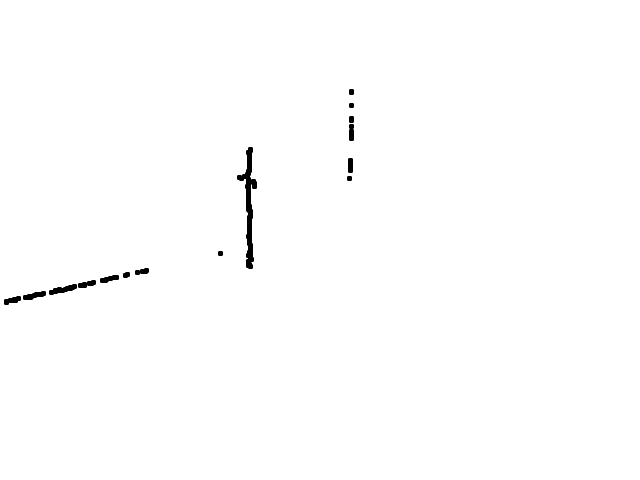
\includegraphics[width=\textwidth]{includes/red_0_diff.png}
		\caption{erkannte Linie nach diff-Linienerkennung}
		\label{fig:red_0_diff}
	\end{subfigure}
	\hfill
	\begin{subfigure}{0.32\textwidth}
		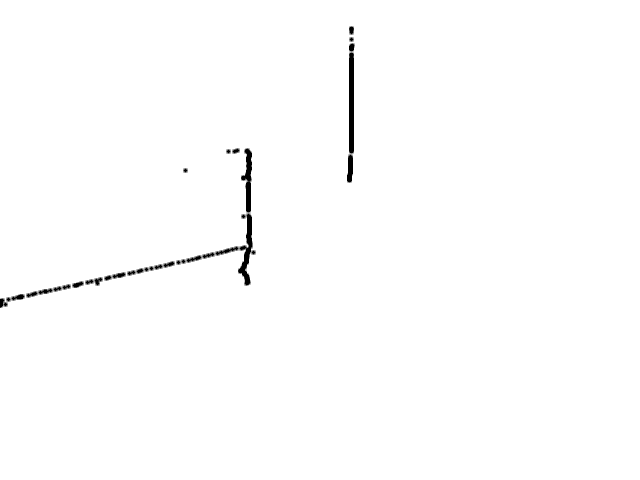
\includegraphics[width=\textwidth]{includes/red_0_free.png}
		\caption{erkannte Linie nach free-Linienerkennung}
		\label{fig:red_0_free}
	\end{subfigure}
	
	\begin{subfigure}{0.32\textwidth}
		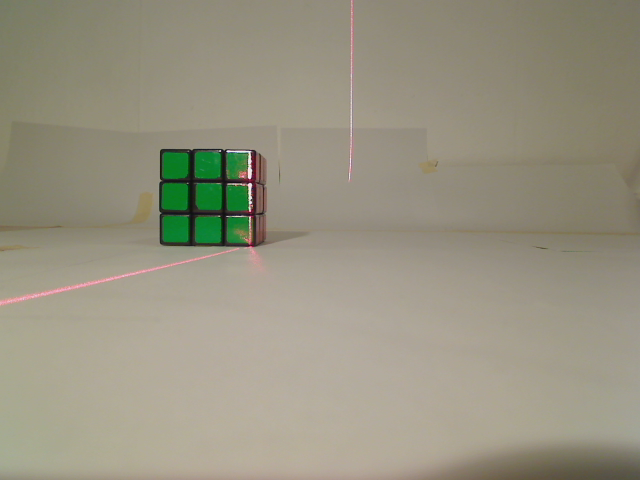
\includegraphics[width=\textwidth]{includes/green_0.png}
		\caption{Bild der Kamera\\}
		\label{fig:green_0_cam}
	\end{subfigure}
	\hfill
	\begin{subfigure}{0.32\textwidth}
		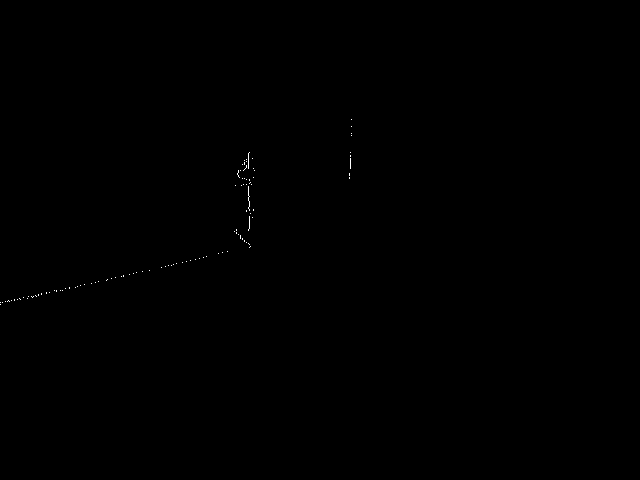
\includegraphics[width=\textwidth]{includes/green_0_diff.png}
		\caption{erkannte Linie nach diff-Linienerkennung}
		\label{fig:green_0_diff}
	\end{subfigure}
	\hfill
	\begin{subfigure}{0.32\textwidth}
		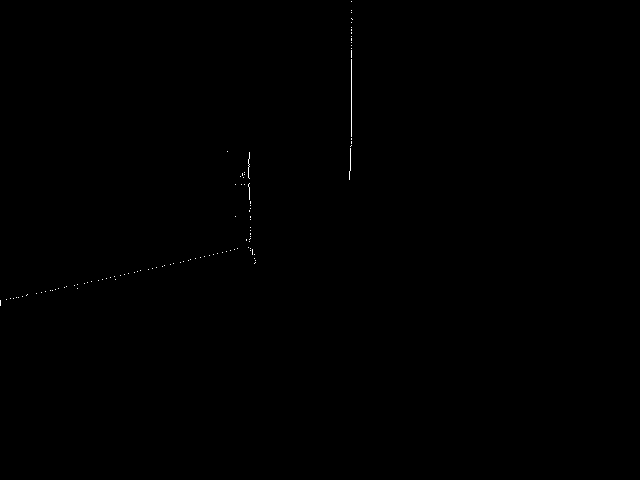
\includegraphics[width=\textwidth]{includes/green_0_free.png}
		\caption{erkannte Linie nach free-Linienerkennung}
		\label{fig:green_0_free}
	\end{subfigure}
	
	\begin{subfigure}{0.32\textwidth}
		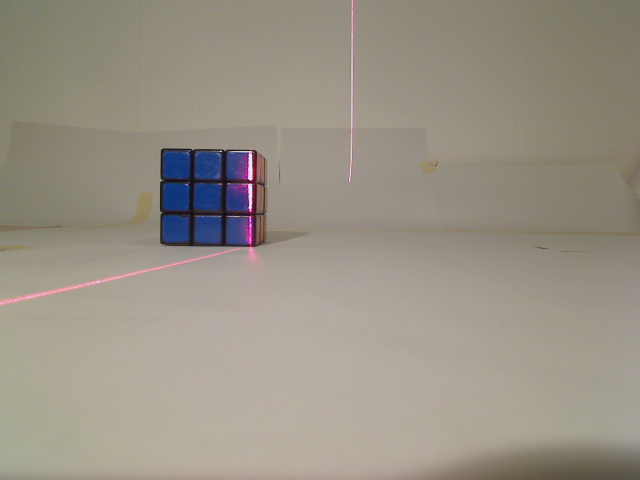
\includegraphics[width=\textwidth]{includes/blue_0.png}
		\caption{Bild der Kamera\\}
		\label{fig:blue_0_cam}
	\end{subfigure}
	\hfill
	\begin{subfigure}{0.32\textwidth}
		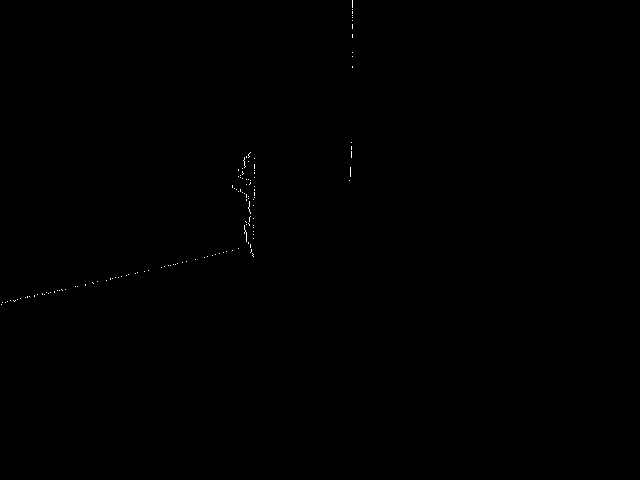
\includegraphics[width=\textwidth]{includes/blue_0_diff.png}
		\caption{erkannte Linie nach diff-Linienerkennung}
		\label{fig:blue_0_diff}
	\end{subfigure}
	\hfill
	\begin{subfigure}{0.32\textwidth}
		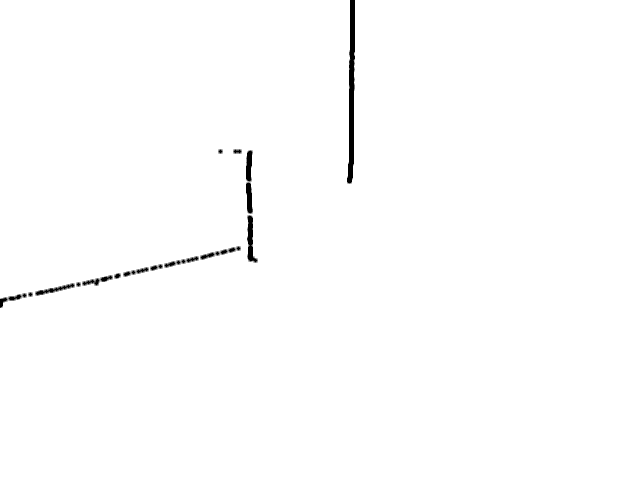
\includegraphics[width=\textwidth]{includes/blue_0_free.png}
		\caption{erkannte Linie nach free-Linienerkennung}
		\label{fig:blue_0_free}
	\end{subfigure}
	
	\begin{subfigure}{0.32\textwidth}
		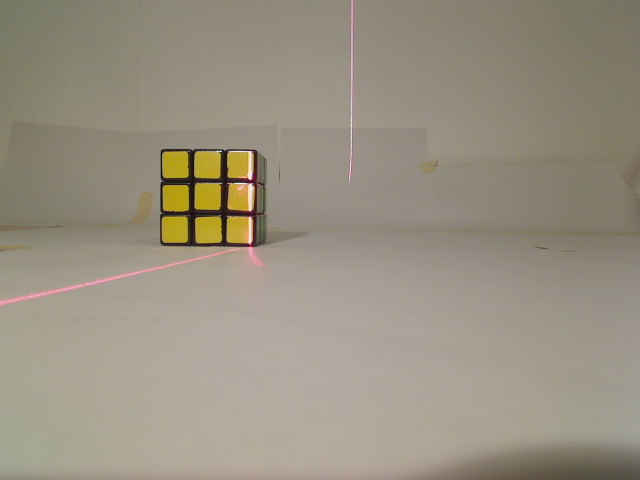
\includegraphics[width=\textwidth]{includes/yellow_0.png}
		\caption{Bild der Kamera\\}
		\label{fig:yellow_0_cam}
	\end{subfigure}
	\hfill
	\begin{subfigure}{0.32\textwidth}
		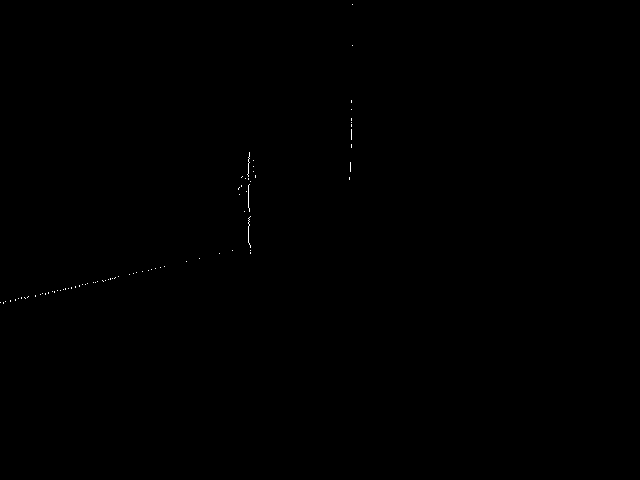
\includegraphics[width=\textwidth]{includes/yellow_0_diff.png}
		\caption{erkannte Linie nach diff-Linienerkennung}
		\label{fig:yellow_0_diff}
	\end{subfigure}
	\hfill
	\begin{subfigure}{0.32\textwidth}
		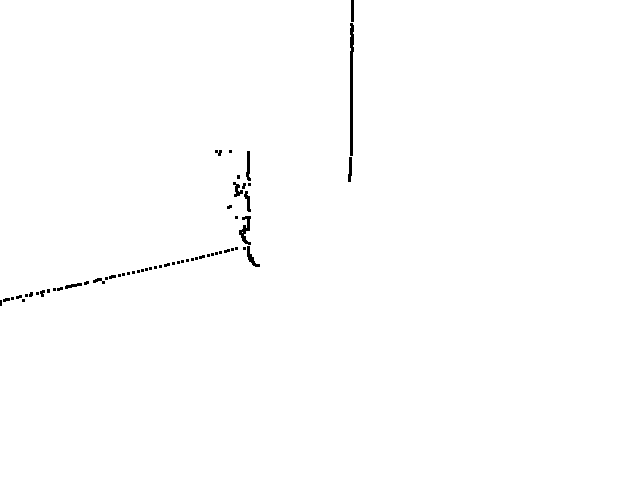
\includegraphics[width=\textwidth]{includes/yellow_0_free.png}
		\caption{erkannte Linie nach free-Linienerkennung}
		\label{fig:yellow_0_free}
	\end{subfigure}
	
	\begin{subfigure}{0.32\textwidth}
		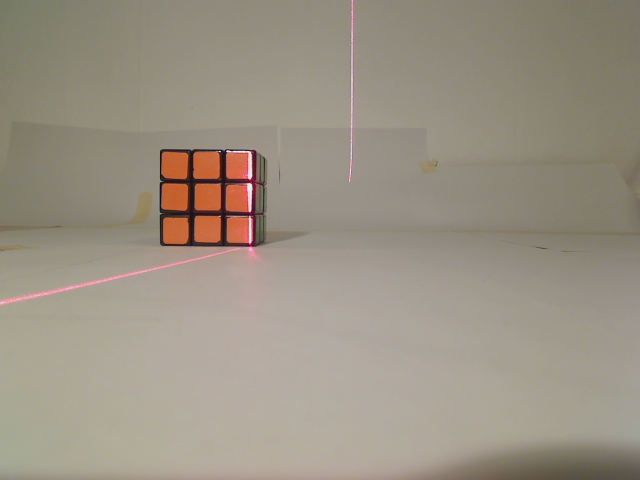
\includegraphics[width=\textwidth]{includes/orange_0.png}
		\caption{Bild der Kamera\\}
		\label{fig:orange_0_cam}
	\end{subfigure}
	\hfill
	\begin{subfigure}{0.32\textwidth}
		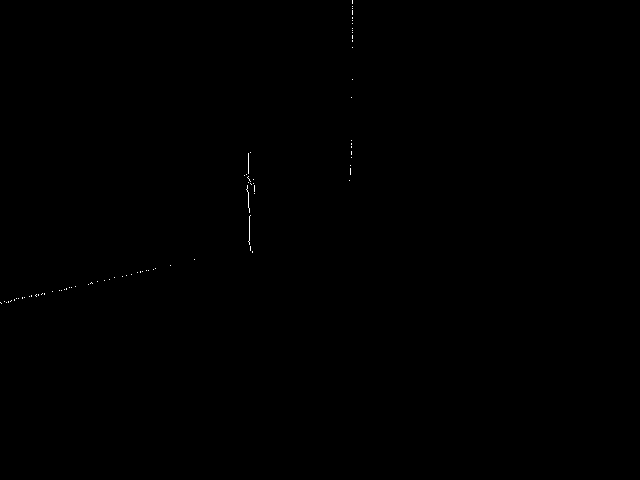
\includegraphics[width=\textwidth]{includes/orange_0_diff.png}
		\caption{erkannte Linie nach diff-Linienerkennung}
		\label{fig:orange_0_diff}
	\end{subfigure}
	\hfill
	\begin{subfigure}{0.32\textwidth}
		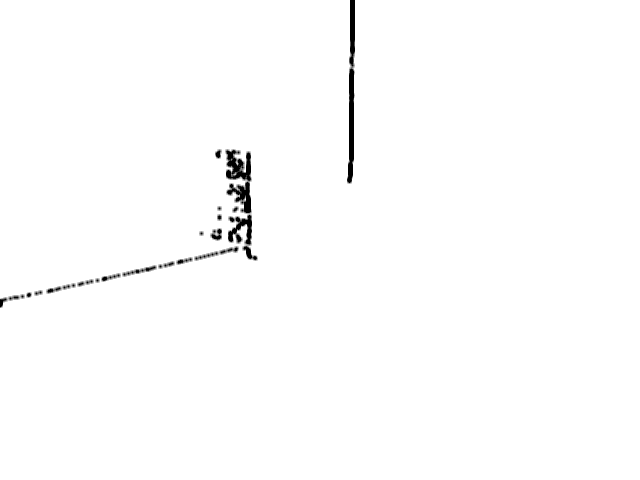
\includegraphics[width=\textwidth]{includes/orange_0_free.png}
		\caption{erkannte Linie nach free-Linienerkennung}
		\label{fig:orange_0_free}
	\end{subfigure}
	\caption{Ergebnisse nach diff- und free-Linienerkennung bei verschiedenen Farben}
	\label{fig:blue_0}
\end{figure}

\subsection{Verschiedene Entfernungen}
\label{sec:dists}

Als drittes wurde die blaue Seite des Würfels in verschiedenen Entfernungen vermessen, um die Entfernungsabhängigkeit der Verfahren zu bestimmen. Die Ergebnisse sind in Tabelle \ref{tab:dists}, die analog zu den vorherigen Tabellen aufgebaut ist, mit dem Unterschied, dass es eine weitere Spalte (''Diff(\%)'') gibt, in der der relative Unterschied zwischen der gemessenen und der erwarteten Entfernung steht.

Beide Linienerkennungen haben bei allen Entfernungen eine relativ geringe Streuung und liefern ähnliche Durchschnittliche Entfernungen, wobei die gemessene Entfernung immer größer ist als die tatsächliche. Eine Ursache ist, dass die angegebene Entfernung der Abstand vom Setup zum Würfel ist, aber die Rekonstruktion die Entfernung vom Brennpunkt der Kamera zum Würfel misst. Das allein würde aber nur eine konstante Abweichung von gemessener und erwarteter Entfernung erklären, da die gemessene Entfernung aber in allen fällen 12\%-17\% größer ist und sogar mit steigender Entfernung größer wird, liegt es nahe, dass es eine weitere Fehlerquelle gibt. Ein schlecht Kalibriertes Setup ist dabei der Wahrscheinlichste Kandidat.

\begin{table}[H]
	\centering
	\begin{tabular}{c|c|c}
		& diff & free \\
		\begin{tabular}{c}
			Entfernung (mm) \\
			\hline
			200 \\
			300 \\
			400 \\
			500 \\
		\end{tabular} & 
		\begin{tabular}{c|c|c|c}
			Anzahl & Avg (mm) & Diff ($\%$) & Stdabw (mm) \\ \hline
			19048 & 224.166 & 12.0 & 8.76011 \\
			8321 & 338.722 & 12.7 & 14.8228 \\
			4294 & 460.079 & 15.0 & 14.5428 \\
			3063 & 587.986 & 17.6 & 11.6962 \\
		\end{tabular} & 
		\begin{tabular}{c|c|c|c}
			Anzahl & Avg (mm) & Diff ($\%$) & Stdabw (mm) \\ \hline
			5733 & 225.367 & 12.5 & 1.08721 \\
			3535 & 340.892 & 13.6 & 2.82819 \\
			1475 & 461.271 & 15.3 & 3.90112 \\
			1156 & 586.405 & 17.3 & 7.37468 \\
		\end{tabular}
	\end{tabular}
	\caption{Scans der blauen Seiten in verschiedenen Entfernungen}
	\label{tab:dists}
\end{table}

\subsection{Verschiedene Beleuchtungen}

Zuletzt wurden die Einflüsse unterschiedlicher Beleuchtungen untersucht. Bisher wurde der ''Rubic's Cube'' direkt von einer Schreibtischlampe und von einer Deckenlampe beleuchtet. Nun wurde einmal die Schreibtischlampe und einmal die Deckenbeleuchtung ausgeschaltet. Der Versuch konnte nicht bei vollständiger Dunkelheit durchgeführt werden, da dabei das Referenzbild komplett schwarz ist, was es unmöglich macht zu unterscheiden, ob ein Messpunkt zur Würfeloberfläche gehört oder nicht. Die Ergebnisse sind in Tabelle \ref{tab:lights} zu sehen.

Wie bereits in Abschnitt \ref{sec:reps} angesprochen, spiegelt sich der Laser im Würfel, was, wie man in den Abbildungen \ref{fig:blue_d_diff}, \ref{fig:blue_t_diff} und \ref{fig:blue_dt_diff} sehen kann, von der diff-Linienerkennung fälschlicherweise als Linie erkannt wird. Bei schwächerer Beleuchtung ist der Spiegeleffekt stärker, was dazu führt, dass diff bei der Beleuchtung nur durch die Deckenlampe schlechtere Ergebnisse liefert, als bei einer direkten Beleuchtung durch die Schreibtischlampe. Beide Lampen zusammen liefern die besten Ergebnisse.

Die free-Linienerkennung wird durch diese Spiegeleffekte nicht beeinflusst, allerdings erkennt sie, wie man in Abbildung \ref{fig:blue_d_free} sehen kann, falsche Punkte auf dem Boden. Die Beleuchtung durch die Schreibtischlampe sorgt dafuer, dass es hellere und dunklere Bereiche in dem Bild gibt. Das führt dazu, dass wie in Abschnitt \ref{sec:cols} der Mittelwert verzerrt wird und auch falsche Punkte erkannt werden

\begin{table}[H]
	\centering
	\begin{tabular}{c|c|c}
		& diff & free \\
		\begin{tabular}{c}
			Beleuchtung \\ \hline
			Schreibtischlampe \\
			Deckenlampe \\
			%Schreibtisch- \\ und \\ Deckenlampe \\
			beides \\
		\end{tabular} & 
		\begin{tabular}{c|c|c}
			Anzahl & Avg (mm) & Stdabw (mm) \\ \hline
			9264 & 338.236 & 34.9526 \\
			12267 & 335.573 & 97.8706 \\
			8321 & 338.722 & 14.8228 \\
		\end{tabular} & 
		\begin{tabular}{c|c|c}
			Anzahl & Avg (mm) & Stdabw (mm) \\ \hline
			4451 & 340.415 & 32.2099 \\
			5890 & 339.616 & 2.99821 \\
			3535 & 340.892 & 2.82819 \\
		\end{tabular}
	\end{tabular}
	\caption{Scans der blauen Seiten in 300mm Entfernungen mit verschiedenen Beleuchtungen}
	\label{tab:lights}
\end{table}

\begin{figure}[H]
	\centering
	\begin{subfigure}{0.32\textwidth}
		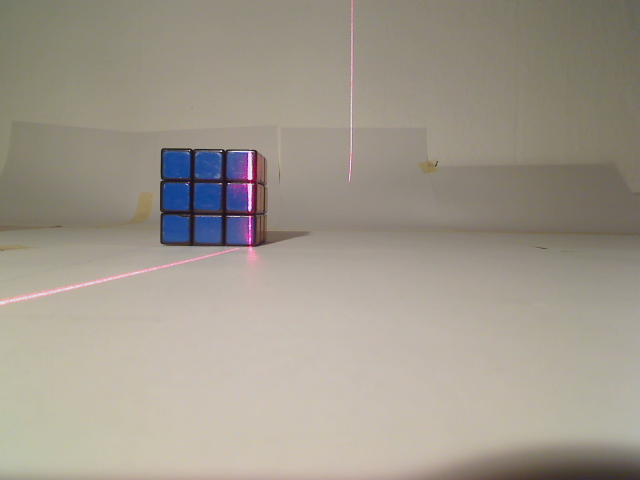
\includegraphics[width=\textwidth]{includes/blue_d.png}
		\caption{Bild der Kamera\\}
		\label{fig:blue_d_cam}
	\end{subfigure}
	\hfill
	\begin{subfigure}{0.32\textwidth}
		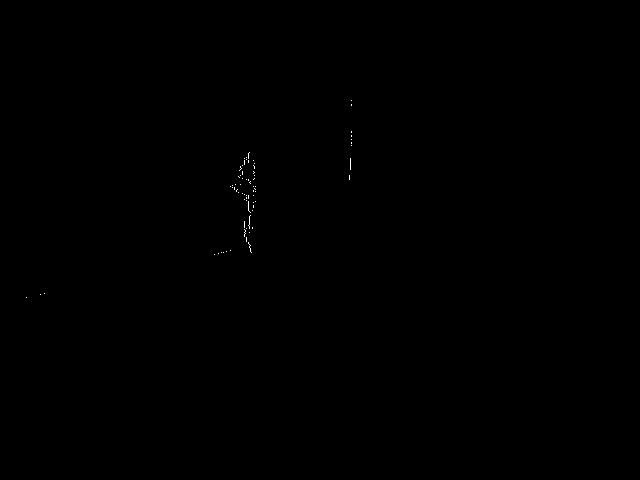
\includegraphics[width=\textwidth]{includes/blue_d_diff.png}
		\caption{erkannte Linie nach diff-Linienerkennung}
		\label{fig:blue_d_diff}
	\end{subfigure}
	\hfill
	\begin{subfigure}{0.32\textwidth}
		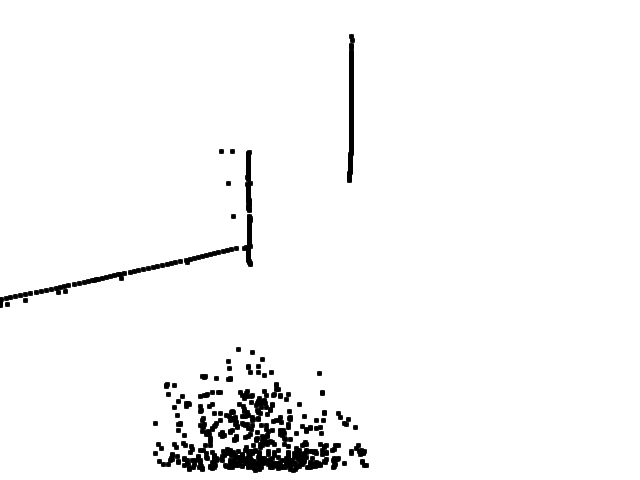
\includegraphics[width=\textwidth]{includes/blue_d_free.png}
		\caption{erkannte Linie nach free-Linienerkennung}
		\label{fig:blue_d_free}
	\end{subfigure}
	\caption{Ergebnisse nach diff- und free-Linienerkennung bei Beleuchtung durch eine Schreibtischlampe}
	\label{fig:blue_d}
\end{figure}

\begin{figure}[H]
	\centering
	\begin{subfigure}{0.32\textwidth}
		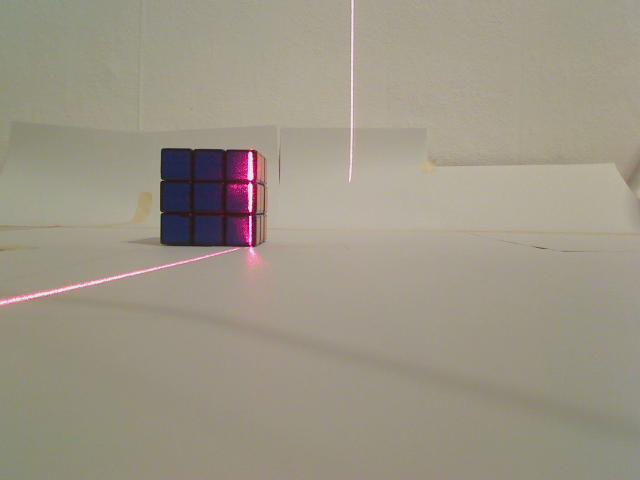
\includegraphics[width=\textwidth]{includes/blue_t.png}
		\caption{Bild der Kamera\\}
		\label{fig:blue_t_cam}
	\end{subfigure}
	\hfill
	\begin{subfigure}{0.32\textwidth}
		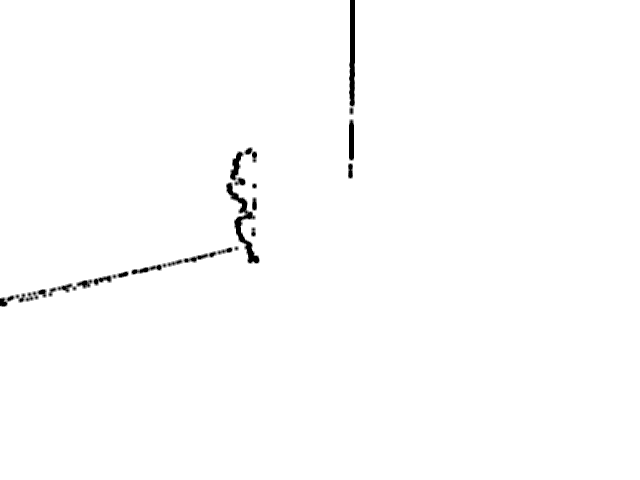
\includegraphics[width=\textwidth]{includes/blue_t_diff.png}
		\caption{erkannte Linie nach diff-Linienerkennung}
		\label{fig:blue_t_diff}
	\end{subfigure}
	\hfill
	\begin{subfigure}{0.32\textwidth}
		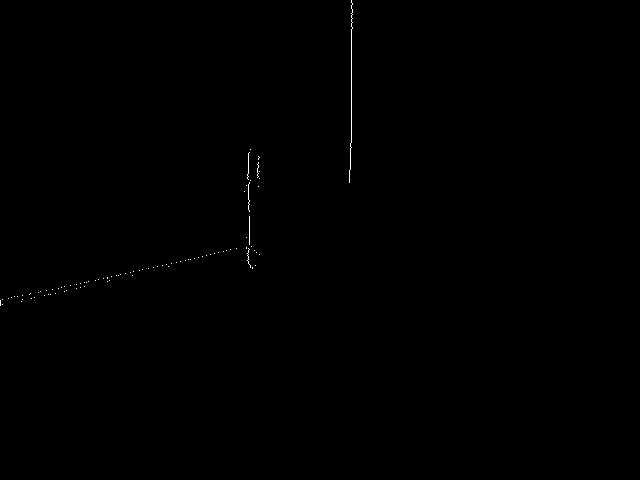
\includegraphics[width=\textwidth]{includes/blue_t_free.png}
		\caption{erkannte Linie nach free-Linienerkennung}
		\label{fig:blue_t_free}
	\end{subfigure}
	\caption{Ergebnisse nach diff- und free-Linienerkennung bei Beleuchtung durch eine Deckenlampe}
	\label{fig:blue_t}
\end{figure}

\begin{figure}[H]
	\centering
	\begin{subfigure}{0.32\textwidth}
		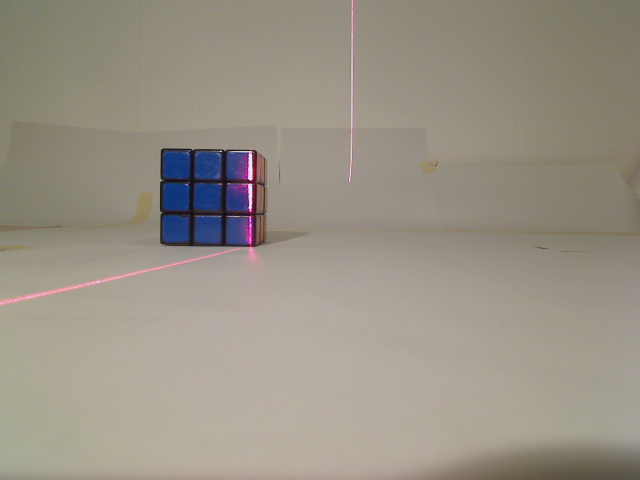
\includegraphics[width=\textwidth]{includes/blue_dt.png}
		\caption{Bild der Kamera\\}
		\label{fig:blue_dt_cam}
	\end{subfigure}
	\hfill
	\begin{subfigure}{0.32\textwidth}
		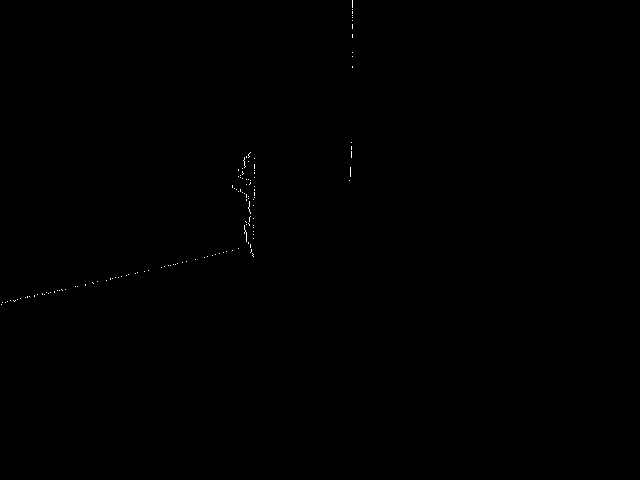
\includegraphics[width=\textwidth]{includes/blue_dt_diff.png}
		\caption{erkannte Linie nach diff-Linienerkennung}
		\label{fig:blue_dt_diff}
	\end{subfigure}
	\hfill
	\begin{subfigure}{0.32\textwidth}
		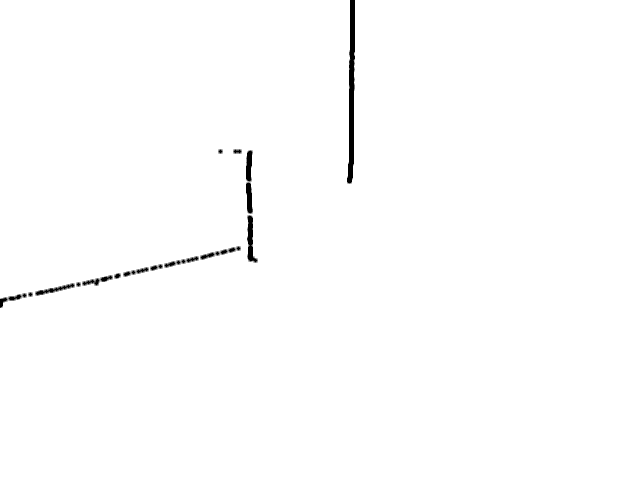
\includegraphics[width=\textwidth]{includes/blue_dt_free.png}
		\caption{erkannte Linie nach free-Linienerkennung}
		\label{fig:blue_dt_free}
	\end{subfigure}
	\caption{Ergebnisse nach diff- und free-Linienerkennung bei Beleuchtung durch Schreibtisch- und Deckenlampe}
	\label{fig:blue_dt}
\end{figure}



% ---------------------------------------------------------------------------- %

\section{Zusammenfassung}
\label{sec:summary}

% ---------------------------------------------------------------------------- %

\section{Quellenverzeichnis}

% ---------------------------------------------------------------------------- %

\end{document}
